\documentclass[
  shownotes,
  xcolor={svgnames},
  hyperref={colorlinks,citecolor=DarkBlue,linkcolor=DarkRed,urlcolor=DarkBlue}
  , aspectratio=169]{beamer}
\usepackage{animate}
\usepackage{amsmath}
\usepackage{amsfonts}
\usepackage{amssymb}
\usepackage{pifont}
\usepackage{mathpazo}
%\usepackage{xcolor}
\usepackage{multimedia}
\usepackage{fancybox}
\usepackage[para]{threeparttable}
\usepackage{multirow}
\setcounter{MaxMatrixCols}{30}
\usepackage{subcaption}
\usepackage{graphicx}
\usepackage{lscape}
\usepackage[compatibility=false,font=small]{caption}
\usepackage{booktabs}
\usepackage{ragged2e}
\usepackage{chronosys}
\usepackage{appendixnumberbeamer}
\usepackage{animate}
\setbeamertemplate{caption}[numbered]
\usepackage{color}
%\usepackage{times}
\usepackage{tikz}
\usepackage{comment} %to comment
%% BibTeX settings
\usepackage{natbib}
\bibliographystyle{apalike}
\bibpunct{(}{)}{,}{a}{,}{,}
\setbeamertemplate{bibliography item}{[\theenumiv]}

% Defines columns for bespoke tables
\usepackage{array}
\newcolumntype{L}[1]{>{\raggedright\let\newline\\\arraybackslash\hspace{0pt}}m{#1}}
\newcolumntype{C}[1]{>{\centering\let\newline\\\arraybackslash\hspace{0pt}}m{#1}}
\newcolumntype{R}[1]{>{\raggedleft\let\newline\\\arraybackslash\hspace{0pt}}m{#1}}


\usepackage{xfrac}


\usepackage{multicol}
\setlength{\columnsep}{0.5cm}

% Theme and colors
\usetheme{Boadilla}

% I use steel blue and a custom color palette. This defines it.
\definecolor{andesred}{HTML}{af2433}

% Other options
\providecommand{\U}[1]{\protect\rule{.1in}{.1in}}
\usefonttheme{serif}
\setbeamertemplate{itemize items}[default]
\setbeamertemplate{enumerate items}[square]
\setbeamertemplate{section in toc}[circle]

\makeatletter

\definecolor{mybackground}{HTML}{82CAFA}
\definecolor{myforeground}{HTML}{0000A0}

\setbeamercolor{normal text}{fg=black,bg=white}
\setbeamercolor{alerted text}{fg=red}
\setbeamercolor{example text}{fg=black}

\setbeamercolor{background canvas}{fg=myforeground, bg=white}
\setbeamercolor{background}{fg=myforeground, bg=mybackground}

\setbeamercolor{palette primary}{fg=black, bg=gray!30!white}
\setbeamercolor{palette secondary}{fg=black, bg=gray!20!white}
\setbeamercolor{palette tertiary}{fg=white, bg=andesred}

\setbeamercolor{frametitle}{fg=andesred}
\setbeamercolor{title}{fg=andesred}
\setbeamercolor{block title}{fg=andesred}
\setbeamercolor{itemize item}{fg=andesred}
\setbeamercolor{itemize subitem}{fg=andesred}
\setbeamercolor{itemize subsubitem}{fg=andesred}
\setbeamercolor{enumerate item}{fg=andesred}
\setbeamercolor{item projected}{bg=gray!30!white,fg=andesred}
\setbeamercolor{enumerate subitem}{fg=andesred}
\setbeamercolor{section number projected}{bg=gray!30!white,fg=andesred}
\setbeamercolor{section in toc}{fg=andesred}
\setbeamercolor{caption name}{fg=andesred}
\setbeamercolor{button}{bg=gray!30!white,fg=andesred}


\usepackage{fancyvrb}
\newcommand{\VerbBar}{|}
\newcommand{\VERB}{\Verb[commandchars=\\\{\}]}
\DefineVerbatimEnvironment{Highlighting}{Verbatim}{commandchars=\\\{\}}
% Add ',fontsize=\small' for more characters per line
\usepackage{framed}
\definecolor{shadecolor}{RGB}{248,248,248}
\newenvironment{Shaded}{\begin{snugshade}}{\end{snugshade}}
\newcommand{\AlertTok}[1]{\textcolor[rgb]{0.94,0.16,0.16}{#1}}
\newcommand{\AnnotationTok}[1]{\textcolor[rgb]{0.56,0.35,0.01}{\textbf{\textit{#1}}}}
\newcommand{\AttributeTok}[1]{\textcolor[rgb]{0.77,0.63,0.00}{#1}}
\newcommand{\BaseNTok}[1]{\textcolor[rgb]{0.00,0.00,0.81}{#1}}
\newcommand{\BuiltInTok}[1]{#1}
\newcommand{\CharTok}[1]{\textcolor[rgb]{0.31,0.60,0.02}{#1}}
\newcommand{\CommentTok}[1]{\textcolor[rgb]{0.56,0.35,0.01}{\textit{#1}}}
\newcommand{\CommentVarTok}[1]{\textcolor[rgb]{0.56,0.35,0.01}{\textbf{\textit{#1}}}}
\newcommand{\ConstantTok}[1]{\textcolor[rgb]{0.00,0.00,0.00}{#1}}
\newcommand{\ControlFlowTok}[1]{\textcolor[rgb]{0.13,0.29,0.53}{\textbf{#1}}}
\newcommand{\DataTypeTok}[1]{\textcolor[rgb]{0.13,0.29,0.53}{#1}}
\newcommand{\DecValTok}[1]{\textcolor[rgb]{0.00,0.00,0.81}{#1}}
\newcommand{\DocumentationTok}[1]{\textcolor[rgb]{0.56,0.35,0.01}{\textbf{\textit{#1}}}}
\newcommand{\ErrorTok}[1]{\textcolor[rgb]{0.64,0.00,0.00}{\textbf{#1}}}
\newcommand{\ExtensionTok}[1]{#1}
\newcommand{\FloatTok}[1]{\textcolor[rgb]{0.00,0.00,0.81}{#1}}
\newcommand{\FunctionTok}[1]{\textcolor[rgb]{0.00,0.00,0.00}{#1}}
\newcommand{\ImportTok}[1]{#1}
\newcommand{\InformationTok}[1]{\textcolor[rgb]{0.56,0.35,0.01}{\textbf{\textit{#1}}}}
\newcommand{\KeywordTok}[1]{\textcolor[rgb]{0.13,0.29,0.53}{\textbf{#1}}}
\newcommand{\NormalTok}[1]{#1}
\newcommand{\OperatorTok}[1]{\textcolor[rgb]{0.81,0.36,0.00}{\textbf{#1}}}
\newcommand{\OtherTok}[1]{\textcolor[rgb]{0.56,0.35,0.01}{#1}}
\newcommand{\PreprocessorTok}[1]{\textcolor[rgb]{0.56,0.35,0.01}{\textit{#1}}}
\newcommand{\RegionMarkerTok}[1]{#1}
\newcommand{\SpecialCharTok}[1]{\textcolor[rgb]{0.00,0.00,0.00}{#1}}
\newcommand{\SpecialStringTok}[1]{\textcolor[rgb]{0.31,0.60,0.02}{#1}}
\newcommand{\StringTok}[1]{\textcolor[rgb]{0.31,0.60,0.02}{#1}}
\newcommand{\VariableTok}[1]{\textcolor[rgb]{0.00,0.00,0.00}{#1}}
\newcommand{\VerbatimStringTok}[1]{\textcolor[rgb]{0.31,0.60,0.02}{#1}}
\newcommand{\WarningTok}[1]{\textcolor[rgb]{0.56,0.35,0.01}{\textbf{\textit{#1}}}}
\usepackage{graphicx}
\makeatletter

\definecolor{airforceblue}{rgb}{0.36, 0.54, 0.66}

\usepackage{tikz}
% Tikz settings optimized for causal graphs.
\usetikzlibrary{shapes,decorations,arrows,calc,arrows.meta,fit,positioning}
\tikzset{
    -Latex,auto,node distance =1 cm and 1 cm,semithick,
    state/.style ={ellipse, draw, minimum width = 0.7 cm},
    point/.style = {circle, draw, inner sep=0.04cm,fill,node contents={}},
    bidirected/.style={Latex-Latex,dashed},
    el/.style = {inner sep=2pt, align=left, sloped}
}


\makeatother






%%%%%%%%%%%%%%% BEGINS DOCUMENT %%%%%%%%%%%%%%%%%%

\begin{document}
 
\title[Lecture 18]{Lecture 18: \\ Classification}
\subtitle{Big Data and Machine Learning for Applied Economics \\ Econ 4676}
\date{\today}

\author[Sarmiento-Barbieri]{Ignacio Sarmiento-Barbieri}
\institute[Uniandes]{Universidad de los Andes}


\begin{frame}[noframenumbering]
\maketitle
\end{frame}

%%%%%%%%%%%%%%%%%%%%%%%%%%%%%%%%%%%



%----------------------------------------------------------------------% 

\begin{frame}
\frametitle{Agenda}

\tableofcontents

\end{frame}

%----------------------------------------------------------------------%
\section{Recap: Regularization and Lasso for Causality }
%----------------------------------------------------------------------%
\begin{frame}[fragile]
\frametitle{Elastic Net}

\begin{itemize}
\item Naive Elastic Net
\end{itemize}

\begin{align}
min_{\beta} NEL(\beta) &= \sum_{i=1}^n (y_i-x_i'\beta)^2 + \lambda_1 \sum_{s=2}^p |\beta_s| + \lambda_2 \sum_{s=2}^p \beta_s^2 
\end{align}

\begin{itemize}
\item Elastic Net: reescaled version. Double Shrinkage introduces ``too'' much bias, {\it final} version ``corrects'' for this
\end{itemize}
\bigskip
\begin{align}
\hat{\beta}_{EN}= \frac{1}{\sqrt{1+\lambda_2}}\hat{\beta}_{naive\,EN}
\end{align}




\end{frame}
%----------------------------------------------------------------------%
\begin{frame}[fragile]
\frametitle{Lasso for Causality}
\framesubtitle{Inference with Selection among Many Controls}

\begin{align}
    y_i = \alpha D_i + X_i'\theta_y +r_{yi} + \zeta_i
  \end{align}

\begin{itemize}
\item We apply variable selection methods to each of the two reduced form equations and then use all of the selected controls in estimation of $\alpha$. 
\medskip
\item We select
\begin{enumerate}
\item A set of variables that are useful for predicting $y_i$, say $X_{yi}$, and 
\item A set of variables that are useful for predicting $D_i$, say $X_{di}$.

\end{enumerate}
\item We then estimate $\alpha$ by ordinary least squares regression of $y_i$ on $d_i$ and the union of the variables selected for predicting $y_i$ and $D_i$, contained in $X_{yi}$ and $X_{di}$. 

\item We thus make sure we use variables that are important for either of the two predictive relationships to guard against OVB

%Using both variable selection steps immunizes the resulting procedure against the types of model selection mistakes discussed above for single-equation procedures. Specififically, using the variables selected in both reduced form equations ensures that any variables that have large effects in either the “structural” equation for yi or the reduced form equation for di are included in the model. Any excluded variables are therefore at most mildly associated to yi and di, which greatly limits the scope for omitted-variables bias. It is also noteworthy that the “double selection” procedure implicitly estimates the residuals εi and vi and then regresses the estimates of εi on the estimates of vi to construct an estimator of α, thereby providing a selection analog of Robinson’s (1988) method for estimating the parameters of a partially linear model to the high-dimensional case.
\end{itemize}
\end{frame}


%----------------------------------------------------------------------%
\section{Classification}
%----------------------------------------------------------------------%
\begin{frame}[fragile]
\frametitle{Classification}


\centering
{\huge \textcolor{andesred}{Classification}}



\end{frame}
%----------------------------------------------------------------------%
\begin{frame}[fragile]
\frametitle{Classification: Motivation}

\begin{itemize}
\item Admit a student to $PEG$ based on their grades and LoR
\medskip
\item Give a credit, based on credit history, demographics?
\medskip
\item Classifying emails: spam, personal, social based on email contents
\medskip
\item Aim is to classify $y$ based on $X's$
\medskip
\item $y$ can be
\begin{itemize}
  \item qualitative (e.g., spam, personal, social)
  \item Not necessarily ordered
  \item Not necessarily two categories, but will start with the binary case

\end{itemize}
\end{itemize}


\end{frame}
%----------------------------------------------------------------------%
\begin{frame}[fragile]
\frametitle{Motivation}

\begin{itemize}
  \item Two states of nature $y \rightarrow n\in\{0,1\}$
  \medskip
  \item Two actions $(\hat{y}) \rightarrow a\in \{0,1\}$
\end{itemize}

%begin{table}[H]
%centering
%begin{tabular}{cccc}
%& \multicolumn{3}{c}{$\hat{y}$}\tabularnewline
%&  & 0 & 1 \\
%\hline
%multirow{2}{*}{y} & 0 & True Negative & False Positive \\
%& 1 & False Negatice & True Positive \\
%end{tabular}
%end{table}


        \begin{figure}[H] \centering
            \captionsetup{justification=centering}
              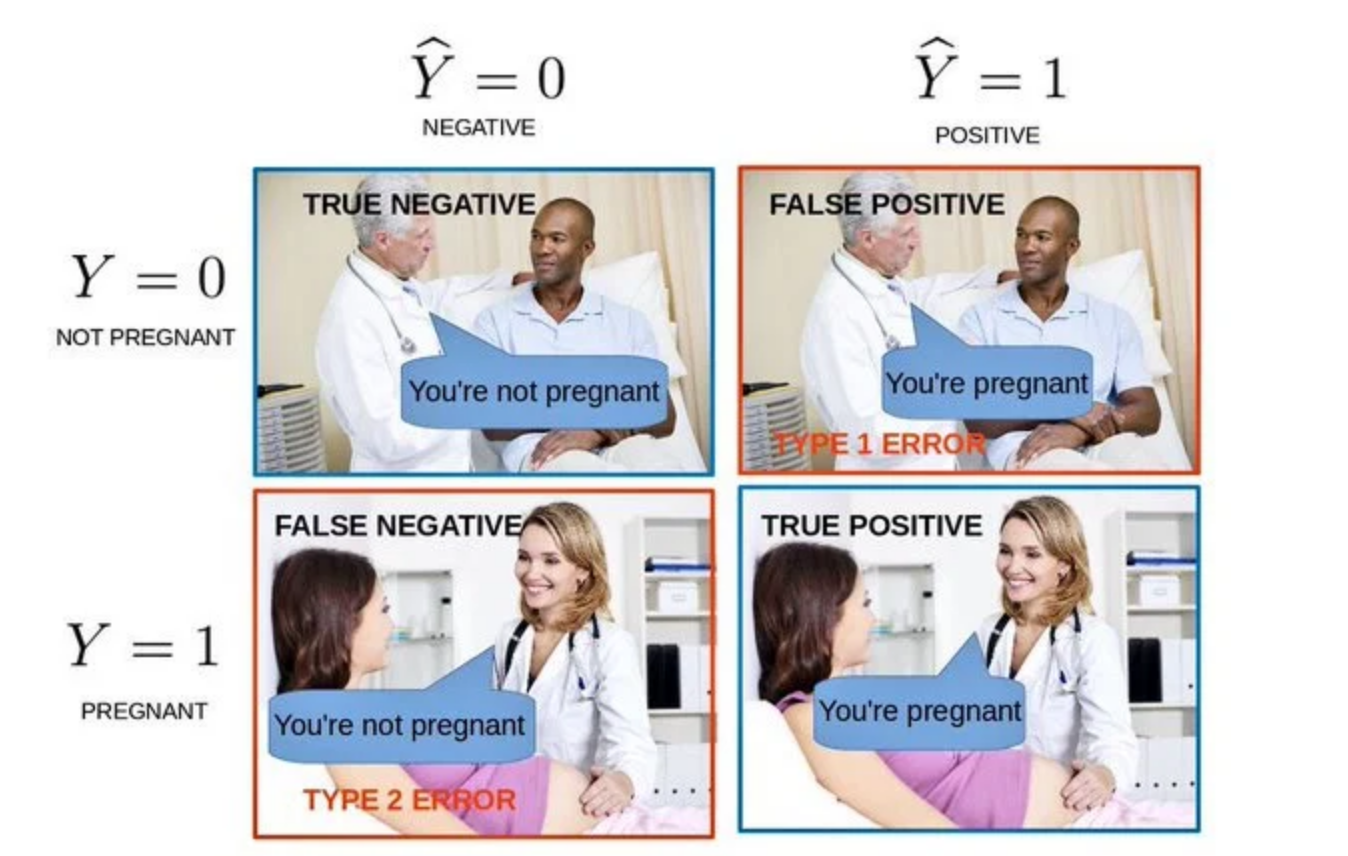
\includegraphics[scale=0.4]{figures/confusion_matrix}
              \\
              \tiny
              Source: \url{https://dzone.com/articles/understanding-the-confusion-matrix}
 \end{figure}

\end{frame}


%----------------------------------------------------------------------%
\begin{frame}[fragile]
\frametitle{Probability, Cost, and Classification}

\begin{itemize}
  \item Two states of nature $y \rightarrow n\in\{0,1\}$
  \medskip
  \item Two actions $(\hat{y}) \rightarrow a\in \{0,1\}$
  \medskip
  \item Probabilities
  \begin{itemize}
    \item $p=Pr(y=1|X)$
    \item $1-p=Pr(y=0|X)$
  \end{itemize}
  \medskip
  \item Loss: $L(a,)$, penalizes being in bin $(a,n)$
  \item Risk: expected loss of taking action $a$
\end{itemize}


\end{frame}
%----------------------------------------------------------------------%
\begin{frame}[fragile]
\frametitle{Probability, Cost, and Classification}

\begin{itemize}
  \item Risk: expected loss of taking action $a$
\end{itemize}

\begin{align}
E[L(a,n)] &= \sum_n p_n L(a,n) \\ \nonumber
R(a) &= (1-p) L(a,0) + p L(a,1)
\end{align}

\begin{itemize}
  \item The objective is the same as before: minimize the risk
  \item We have to define $L(a,n)$
\end{itemize}

\end{frame}
%----------------------------------------------------------------------%
\begin{frame}[fragile]
\frametitle{Probability, Cost, and Classification}

\begin{itemize}
  \item Which action do we choose?
 \bigskip
 \pause
  \item We can compare the risk of each action
  \medskip
  \item We are going to choose to take action 1 when the risk is lower:
\end{itemize}

\begin{align}
R(1) &< R(0) \\ \nonumber
1-p &< p \\ \nonumber
p &> \frac{1}{2} \\ \nonumber
\end{align}

\begin{itemize}
  \item This is known as the Bayes Classifier, choose the estate that minimizes the risk
\end{itemize}

\end{frame}
%----------------------------------------------------------------------%
\begin{frame}[fragile]
\frametitle{Probability, Cost, and Classification}

\begin{itemize}
  \item Under a 0-1 penalty the problem boils down to finding $p=Pr(y=1|X)$
  \medskip
  \item We then predict 1 if $p>0.5$ and 0 otherwise (Bayes classifier)
  \medskip
  \item We can think 3 ways of finding this probability in binary cases
  \begin{itemize}
    \item K-Nearest Neighbors
    \item Logistic
    \item LDA
  \end{itemize}
\medskip
  \item Why not $p=X\beta$?
\end{itemize}


\end{frame}
%----------------------------------------------------------------------%
\subsection{K-Nearest Neighbors}
%----------------------------------------------------------------------%
\begin{frame}[fragile]
\frametitle{K-Nearest Neighbors}


\centering
{\huge \textcolor{andesred}{K-Nearest Neighbors}}



\end{frame}
%----------------------------------------------------------------------%
\begin{frame}[fragile]
\frametitle{K-Nearest Neighbors}

\begin{itemize}
\item K nearest neighbor (K-NN) algorithm predicts class $\hat y$ for $x$ by asking \\
{\it What is the most common class for observations around x?}
\end{itemize}
        \begin{figure}[H] \centering
            \captionsetup{justification=centering}
              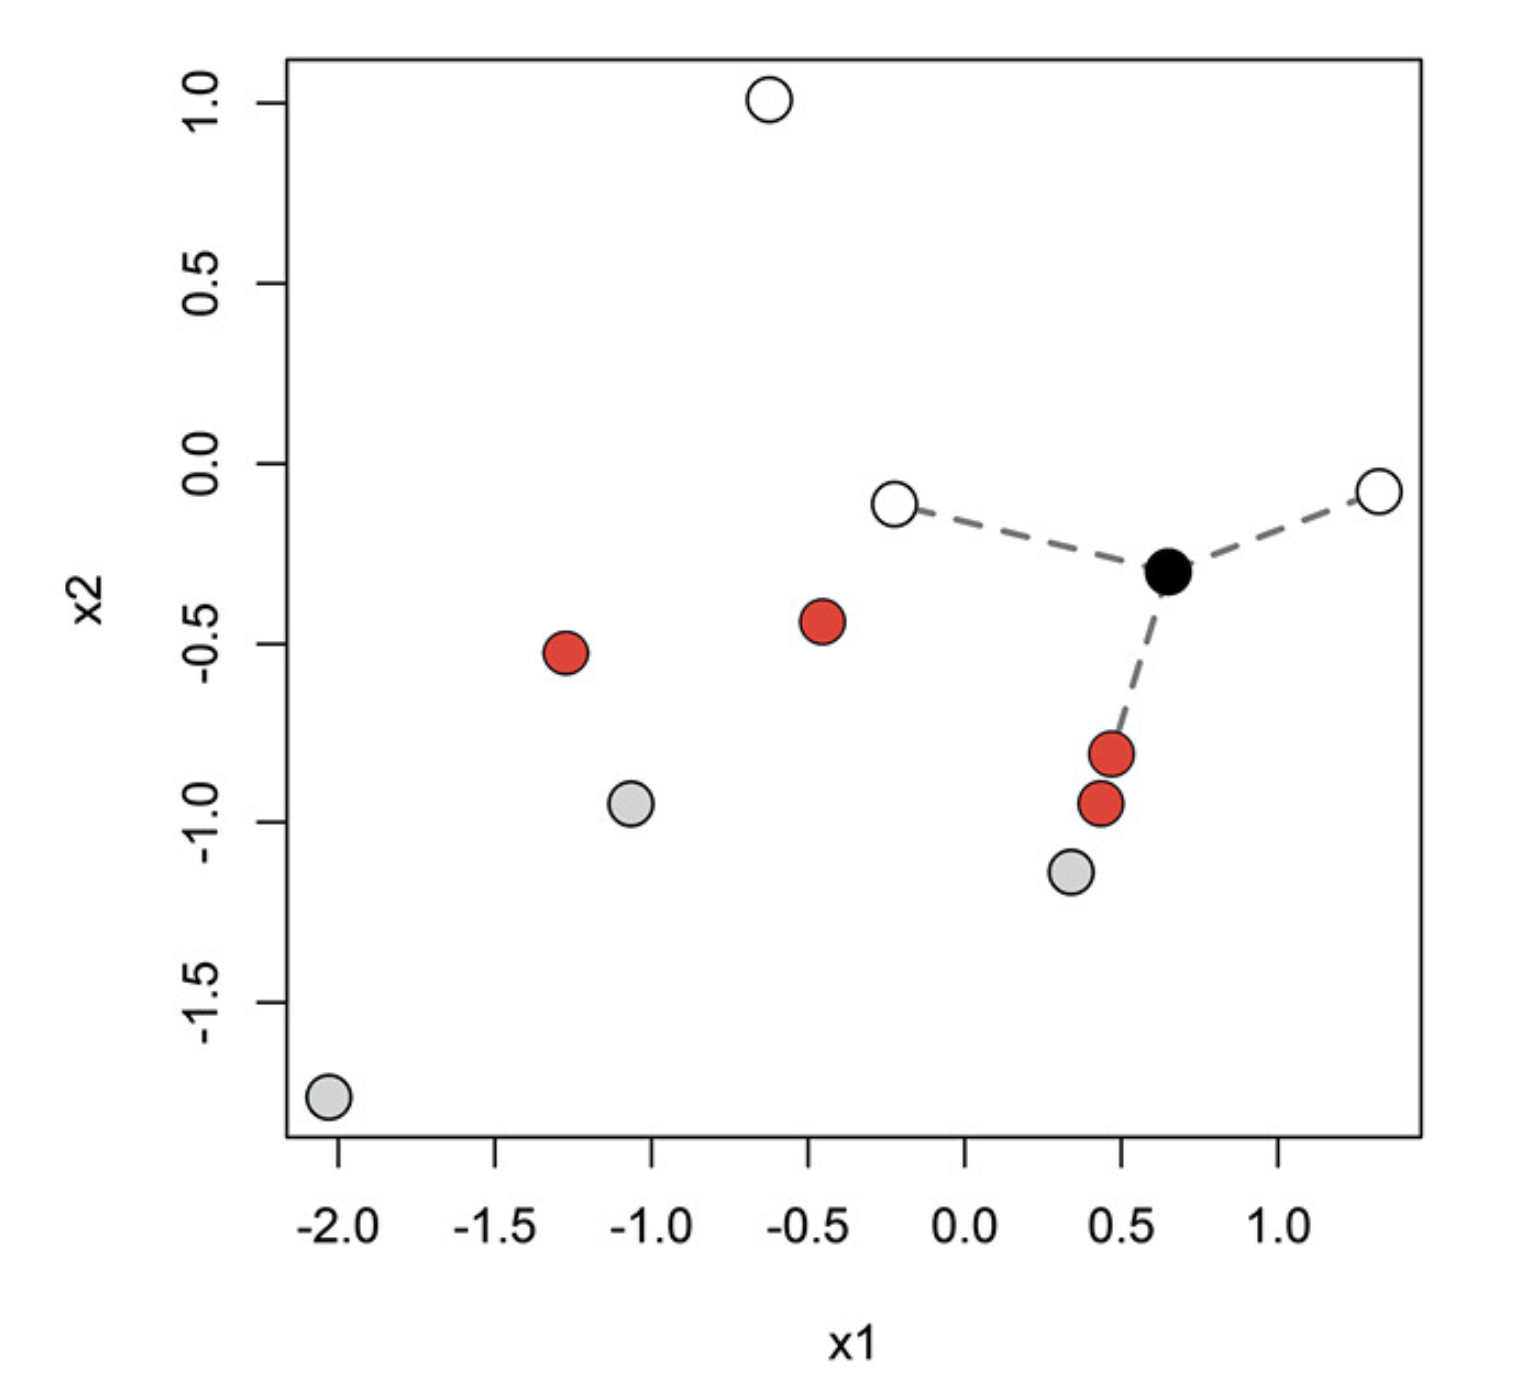
\includegraphics[scale=0.13]{figures/knn}
              \\
              \tiny
              Source: Taddy (2019)
 \end{figure}

 \end{frame}
%----------------------------------------------------------------------%
\begin{frame}[fragile]
\frametitle{K-Nearest Neighbors}

\begin{itemize}
\item K nearest neighbor (K-NN) algorithm predicts class $\hat y$ for $x$ by asking \\
{\it What is the most common class for observations around x?}
\item Algorithm: given an input vector $x_f$ where you would like to predict the class label

\begin{itemize}
  \item Find the K nearest neighbors in the dataset of labeled observations, ${x_i,y_i}_{i=1}^n$, the most common distance is the Euclidean distance (units):
  \begin{align}
  d(x_i,x_f)=\sqrt{\sum_{j=1}^p(x_{ij}-x_{fj})^2}
  \end{align}
  \item This yields a set of the $K$ nearest observations with labels: 
  \begin{align}
  [x_{i1},y_{i1}],\dots,[x_{iK},y_{iK}]
  \end{align}
  \item The predicted class of $x_f$ is the most common class in this set
  \begin{align}
  \hat{y}_f =mode\{y_{i1},\dots,y_{iK}\}
  \end{align}
\end{itemize}

\end{itemize}
\end{frame}

%----------------------------------------------------------------------%
\begin{frame}[fragile]
\frametitle{K-Nearest Neighbors}
\begin{itemize}
  \item There are some major problems with practical applications
  \medskip
  \begin{itemize}
  \item Knn predictions are unstable as a function of $K$
    \end{itemize}
\end{itemize}
  \begin{columns}[T] % align columns
\begin{column}{.58\textwidth}
\begin{align}
  K&=1 \implies \hat{p}(white)=0 \nonumber \\
  K&=2 \implies \hat{p}(white)=1/2 \nonumber \\
  K&=3 \implies \hat{p}(white)=2/3 \nonumber \\
  K&=4 \implies \hat{p}(white)=1/2 \nonumber 
  \end{align}


\end{column}
\hfill
\begin{column}{.4\textwidth}
\begin{figure}[H] \centering
            \captionsetup{justification=centering}
              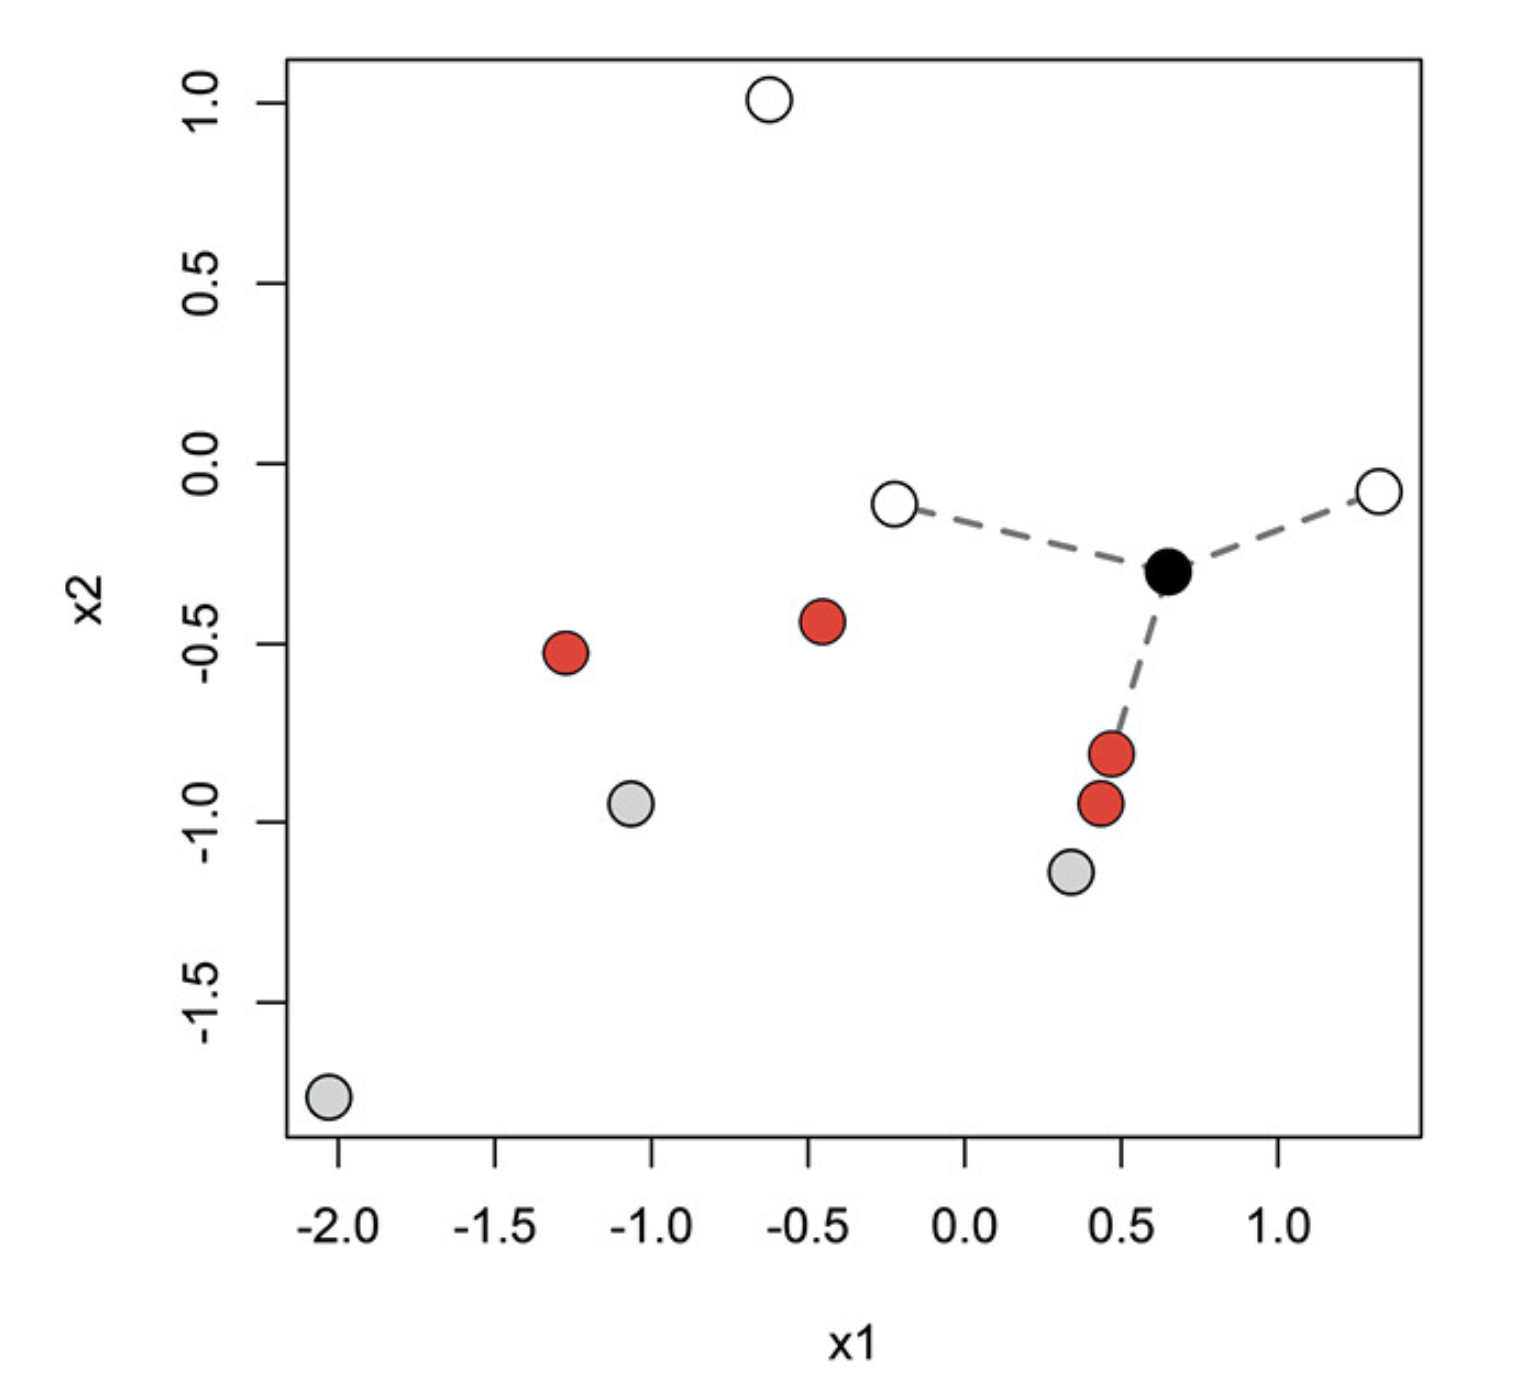
\includegraphics[scale=0.1]{figures/knn}
              \\
              \tiny
              Source: Taddy (2019)
 \end{figure}
\end{column}
\end{columns}
  
\end{frame}


%----------------------------------------------------------------------%
\begin{frame}[fragile]
\frametitle{K-Nearest Neighbors}
\begin{itemize}
\item In this case
  \begin{itemize}
    \item 1-Knn manages 70\% accuracy
    \item 5-Knn manages 60\% accuracy
    \item H.W. try for different seed, (Taddy's is 80\% and 70\%)
  \end{itemize}
  \medskip
  \item There are some major problems with practical implications
  \begin{itemize}
  \item Knn predictions are unstable as a function of $K$
  \medskip
  \item This instability of prediction makes it hard to choose the optimal K and cross validation doesn't work well for KNN
  \medskip
  \item Since prediction for each new $x$ requires a computationally intensive counting, KNN is too expensive to be useful in most big data settings.
  \medskip
  \item KNN is a good idea, but too crude to be useful in practice
  \end{itemize}
\end{itemize}

\end{frame}
%----------------------------------------------------------------------%
\subsection{Logit}
%----------------------------------------------------------------------%
\begin{frame}[fragile]
\frametitle{Logit}


\centering
{\huge \textcolor{andesred}{Logit}}



\end{frame}
%----------------------------------------------------------------------%
\begin{frame}[fragile]
\frametitle{Logit}
We have a conditional probability
\begin{align}
Pr(y=1|X) &= f(X'\beta) 
\end{align}

Logistic regression uses a $logit$ (sigmoid, softmax) link function

\begin{align}
log \left(\frac{p(y=1|X)}{1-p(y=1|X)}\right)=\beta_0 +\beta_1 x_1 + \dots +\beta_k x_k
\end{align}

\end{frame}
%----------------------------------------------------------------------%
\begin{frame}[fragile]
\frametitle{Logit}



        \begin{figure}[H] \centering
            \captionsetup{justification=centering}
              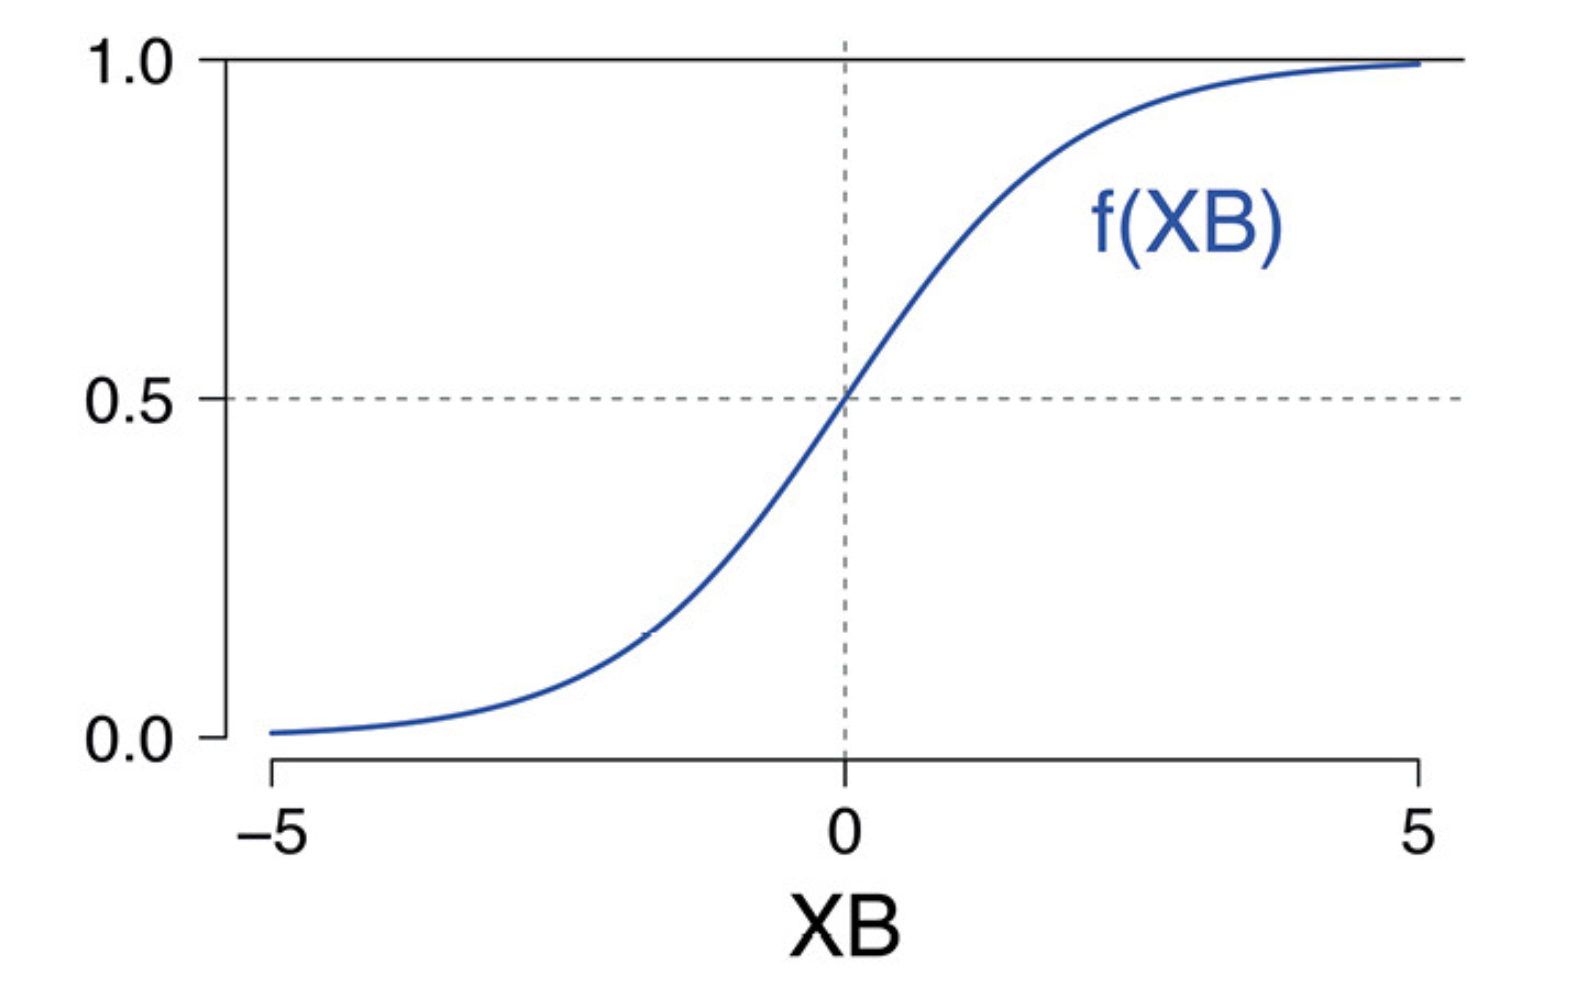
\includegraphics[scale=0.2]{figures/logistic}
              \\
              \tiny
              Source: Taddy (2019)
 \end{figure}

\end{frame}
%----------------------------------------------------------------------%
\begin{frame}[fragile]
\frametitle{Logit}
We have a conditional probability
\begin{align}
Pr(y=1|X) &= f(X'\beta) 
\end{align}

Can recover predictions:

\begin{align}
p(y=1|X)=\frac{e^{X'\beta}}{1+e^{X'\beta}}=\frac{exp(\beta_0 +\beta_1 x_1 + \dots +\beta_k x_k)}{1+exp(\beta_0 +\beta_1 x_1 + \dots +\beta_k x_k)}
\end{align}

\end{frame}

%----------------------------------------------------------------------%
\subsection{Linear Discriminant Analysis}
%----------------------------------------------------------------------%
\begin{frame}[fragile]
\frametitle{Linear Discriminant Analysis}


\centering
{\huge \textcolor{andesred}{Linear Discriminant Analysis}}


\end{frame}
%----------------------------------------------------------------------%
\begin{frame}[fragile]
\frametitle{Linear Discriminant Analysis}
\framesubtitle{Reverend Bayes to the rescue: Bayes Theorem}

\bigskip
\begin{align}
p (y=1|X)=\frac{f(X|y=1)p(y=1)}{m(X)}
\end{align}

\bigskip
with $m(X)$ is the marginal distribution of $X$, i.e.

\begin{align}
m(X)=\int f(X|y=1)p(y=1)dy
\end{align}
Recall that there are two states of nature $y \rightarrow i\in\{0,1\}$
\begin{align}
m(X) &= f(X|y=1)p(y=1) + f(X|y=0)p(y=0) \nonumber \\
    &= f(X|y=1)p(y=1) + f(X|y=0)(1-p(y=1))
\end{align}

\end{frame}
%----------------------------------------------------------------------%
\begin{frame}[fragile]
\frametitle{Linear Discriminant Analysis}
\begin{itemize}
  \item This is basically an empirical Bayes approach
  \item We need to estimate $f(X|y=1)$,  $f(X|y=0)$ and $p(y=1)$ 
  \begin{itemize}
    \item Let's start by estimating $p(y=1)$. We've done this before
    \begin{align}
    p(y=1) = \frac{\sum_{i=1}^n 1[y_i=1]}{N}
    \end{align}
    \item Next $f(X|y=j)$ with $j=0,1$. 
    \begin{itemize}
    \item if we assume one predictor and $X|y\sim N(\mu_j,\sigma_j)$
    \item the problem boils down to estimating $\mu_j,\sigma_j$
    \item LDA makes it simpler, assumes $\sigma_j=\sigma$ $\forall j$
    \item then partition the sample in two $y=0$ and $y=1$, estimate the moments and get $\hat{f}(X|y=j)$
    \end{itemize}
    \item Plug everything into the Bayes Rule and you're done
    

  \end{itemize}
\end{itemize}


\end{frame}
%----------------------------------------------------------------------%
\begin{frame}[fragile]
\frametitle{Linear Discriminant Analysis}
\framesubtitle{Extensions}

\begin{itemize}
    \item If we have $k$ predictors?
    \medskip
    \item then $X|y\sim NM(\mu,\Sigma)$
    \begin{align}
    f(X|y=j) = \frac{1}{(2\pi)^{k/2}|\Sigma|^{1/2}}exp(-\frac{1}{2}(x-\mu_j)'\Sigma_j(x-\mu_j)
    \end{align}
    \item $\mu_j$ is the vector of the sample means in each partition $j=0,1$
    \medskip
    \item $\Sigma_j$ is the matrix of variance and covariances of each partition $j=0,1$
    \medskip
    \item Can we lift normality? 
    \end{itemize}
\end{frame}
%----------------------------------------------------------------------%
\begin{frame}[fragile]
\frametitle{Linear Discriminant Analysis}

\begin{itemize}
  \item Why is it call linear?
  \item Note
  \begin{align}
    p>\frac{1}{2} \iff ln(\frac{p}{(1-p)})
  \end{align}
  \item Logit with one predictor
  \begin{align}
  \beta_1 + \beta_2 X
  \end{align}
  \item Classification: in the probability of space
  \item Discrimination: in the space of X
  \item $\beta_1 +\beta_2 X$ is the discrimination function for logit (it is lineal)
\end{itemize}

\end{frame}
%----------------------------------------------------------------------%
\begin{frame}[fragile]
\frametitle{Linear Discriminant Analysis}
\begin{itemize}
  \item LDA?
  \item One predictor with $\sigma_0 = \sigma_1$ (equal variance)
  \begin{align}
  p (y=1|X)=\frac{f(X|y=1)p(y=1)}{f(X|y=1)p(y=1) + f(X|y=0)(1-p(y=1))}
  \end{align}
  \item Then under the equal variance assumption
  \begin{align}
  \frac{p (y=1|X)}{1-p (y=1|X} &= \frac{f(X|y=1)p(y=1)}{f(X|y=0)(1-p(y=1))} \\
                                &= \frac{p(y=1)exp((x-\mu_1)^2)}{(1-p(y=1))exp((x-\mu_0)^2)} 
  \end{align}
\end{itemize}

\end{frame}
%----------------------------------------------------------------------%
\begin{frame}[fragile]
\frametitle{Linear Discriminant Analysis}
\begin{itemize}
  \item Taking logs

\begin{align}
  log \left( \frac{p (y=1|X)}{1-p (y=1|X}\right)  &= log(\frac{p(y=1)}{(1-p(y=1))}+(x-\mu_1)^2-(x-\mu_0)^2 \\
  &= log(\frac{p(y=1)}{(1-p(y=1))}+\mu^2_1-\mu^2_0-2(\mu_1-\mu_0)x \\
  &= \gamma_1 +\gamma_2 X
  \end{align}  
  \item under the assumption of equal variance the discrimination function is lineal
  \item Note: logit estimates $\gamma_1$ and $\gamma_2$
\end{itemize}

\end{frame}
%----------------------------------------------------------------------%
\section{Misclassification Rates}
%----------------------------------------------------------------------%
\begin{frame}[fragile]
\frametitle{Misclassification Rates}


\centering
{\huge \textcolor{andesred}{Misclassification Rates}}


\end{frame}
%----------------------------------------------------------------------%
\begin{frame}[fragile]
\frametitle{Misclassification Rates}

\begin{itemize}
  \item Predicted probabilities from Logit model
\end{itemize}

\begin{figure}[H] \centering
            \captionsetup{justification=centering}
              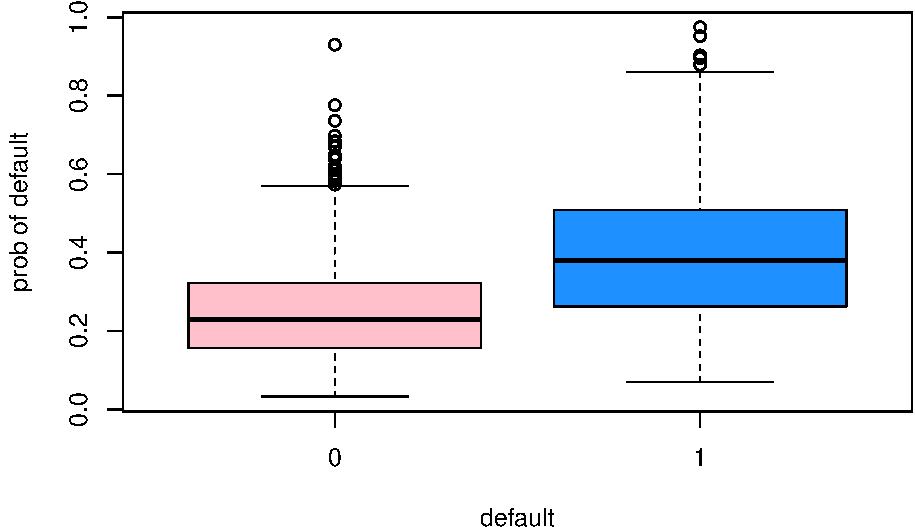
\includegraphics[scale=0.6]{figures/box_plots}                            
 \end{figure}


\end{frame}
%----------------------------------------------------------------------%
\begin{frame}[fragile]
\frametitle{Misclassification Rates}




\begin{columns}[T] % align columns
\begin{column}{.52\textwidth}
\begin{itemize}
  \item A classification rule, or cutoff, is the probability $p$ at which you predict
  \medskip
  \begin{itemize}
    \item $\hat y_i =0$ if $p_i < p$
    \item $\hat y_i = 1$ if $p_i < p$
  \end{itemize}
  \medskip

  \item Measures of performance
  \begin{itemize}
  \item {\it 1-Specificity:} False Positive Rate, Type I error
  \item {\it Sensitivity:} True Positive Rate, power, (1-Type II error)
  \end{itemize}
  
\end{itemize}
\end{column}  
\hfill
\begin{column}{.48\textwidth}

 \begin{figure}[H] \centering
            \captionsetup{justification=centering}
              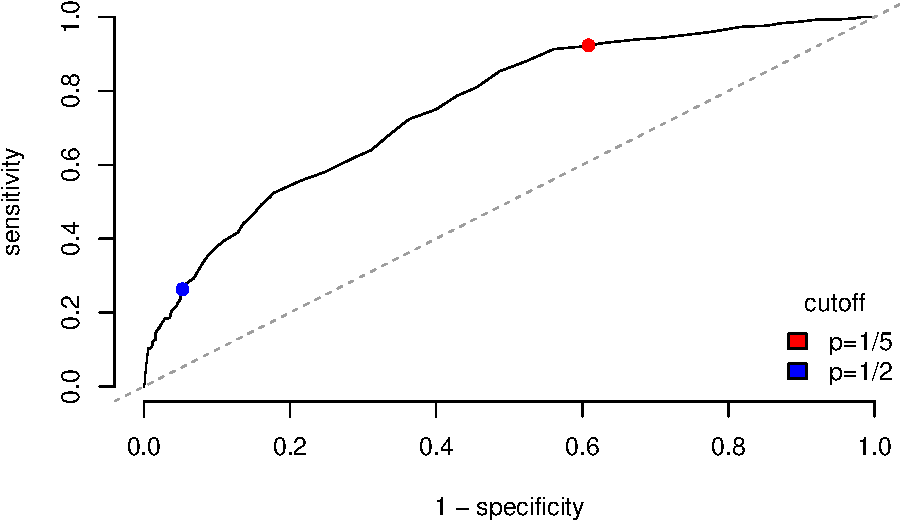
\includegraphics[scale=0.4]{figures/roc}                            
 \end{figure}

\end{column}
\end{columns}

\end{frame}
%----------------------------------------------------------------------%
\subsection{ROC curve}
%----------------------------------------------------------------------%
\begin{frame}[fragile]
\frametitle{ROC}


\begin{itemize}
\item ROC curve: Receiver operating characteristic curve
\medskip
\item ROC curve illustrates the trade-off of the classification rule
\medskip
\item Gives us the ability
\begin{itemize}
  \item Measure the predictive capacity of our model
  \medskip
  \item Compare between models
  \medskip
\end{itemize}
  \item Some definitions
  \begin{itemize}
    \item $P=\sum y_i$ positives
    \medskip
    \item $N=\sum(1-y_i)$ negatives
    \medskip
    \item $T=P+N$ all observations
    \medskip
    \item True Positives: $TP=\sum \hat{y}_i y_i$, True Positive Rate = $\frac{TP}{P}$
    \medskip
    \item False Positives: $FP=\sum \hat{y}_i (1-y_i)$, False Positive Rate = $\frac{FP}{N}$

  \end{itemize}
\end{itemize}


\end{frame}
%----------------------------------------------------------------------%
\begin{frame}[fragile]
\frametitle{ROC}

\begin{columns}[T] % align columns
\begin{column}{.52\textwidth}
  \begin{itemize}
    \item Binary Classifier: $\hat{y}_i=1[p_i>c]$, $c\in[0,1]$
    \medskip
    \item Bayes fixes $c=0.5$
    \medskip
    \item Ideally $TPR=1$  and $FPR=0$
    \medskip
    \item ROC curve give us the locus of all possible $TPR$ and $FPR$ for all possible $c\in[0,1]$
  \end{itemize}
\end{column}  
\hfill
\begin{column}{.48\textwidth}

 \begin{figure}[H] \centering
            \captionsetup{justification=centering}
              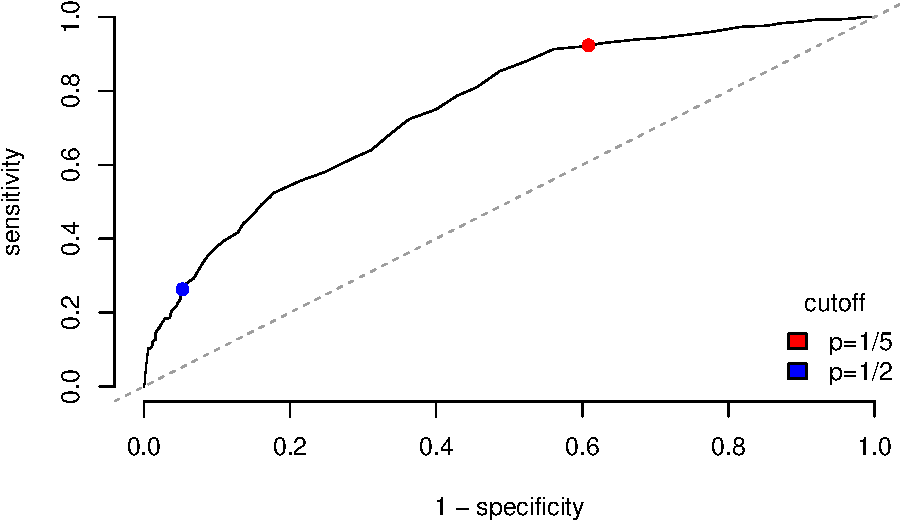
\includegraphics[scale=0.4]{figures/roc}                            
 \end{figure}

\end{column}
\end{columns}

\end{frame}
%----------------------------------------------------------------------%
\begin{frame}[fragile]
\frametitle{ROC}
\begin{itemize}
  \item ROC Properties 

  \begin{itemize}
  \item Has positive slope
  \begin{itemize}
    \item In $(0,0)$, $c=1$. When $c\downarrow$, $TP \uparrow$ and $FP\uparrow$. Then
    \begin{align}
    TPR = \sum \frac{\hat{y}_iy_i}{P} \,\,\,\, FPR = \sum \frac{\hat{y}_i(1-y_i)}{T-P}
    \end{align}
    \item Is easy to show
    \begin{align}
    TPR &= \frac{\sum \hat{y}_i}{P} - \frac{T-P}{P}FPR
    \end{align}
    \item ROC is the locus of all possible $TPR$ and $FPR$ for all possible $c\in[0,1]$ 
    \begin{align}
    TPR &= \frac{\sum \hat{y}_i(c)}{P} - \frac{T-P}{P}FPR(c)
    \end{align}
  \end{itemize}
\end{itemize}  
\end{itemize}




\end{frame}
%----------------------------------------------------------------------%
\begin{frame}[fragile]
\frametitle{ROC: Summary}

\begin{itemize}
  \item Ideal ROC curve
  \medskip
  \item AUC: area under the curve, is like an $R^2$
  \medskip
  \item Help us compare between classifiers
  \medskip
  \item Dominated classifiers?
  \medskip
  \item Which c? Choose a max $FPR$

\end{itemize}

\end{frame}


%----------------------------------------------------------------------%
\section{Review
 \& Next Steps}
%----------------------------------------------------------------------%
\begin{frame}
\frametitle{Review \& Next Steps}
  
\begin{itemize} 
    \item Review Classification:
    \medskip
    \begin{itemize} 
      \item KNN
        \begin{itemize}  
            \item Intuitive
            \item Not very useful in practice, curse of dimensionality
        \end{itemize}      
     \medskip   
    \item Logit
    \medskip
  \item Linear Discriminant Analysis
  \medskip
  \item  Misclassification Rates: ROC curve
  \medskip
  \item QDA?
  \medskip 
  \item Multiple Classes?

    \end{itemize}
    \bigskip  
  \item  Next class:  Problem Sets, Text Data!


\bigskip  
\item Questions? Questions about software? 

\end{itemize}
\end{frame}
%----------------------------------------------------------------------%
\section{Further Readings}
%----------------------------------------------------------------------%
\begin{frame}
\frametitle{Further Readings}

\begin{itemize}


  \item Friedman, J., Hastie, T., \& Tibshirani, R. (2001). The elements of statistical learning (Vol. 1, No. 10). New York: Springer series in statistics.
  \medskip
  \item James, G., Witten, D., Hastie, T., \& Tibshirani, R. (2013). An introduction to statistical learning (Vol. 112, p. 18). New York: springer.
  \medskip
  \item Kuhn, M. (2012). The caret package. R Foundation for Statistical Computing, Vienna, Austria. \url{https://topepo.github.io/caret/index.html}
  \medskip
  \item Taddy, M. (2019). Business data science: Combining machine learning and economics to optimize, automate, and accelerate business decisions. McGraw Hill Professional.
  \medskip
  \item  Zou, H. y Hastie, T., 2005, Regularization and variable selection via the elastic net, Journal of the Royal Statistical Society, 67, 2, 301-320.
  
\end{itemize}

\end{frame}

%----------------------------------------------------------------------%
%----------------------------------------------------------------------%
\section{Demos in R}
%----------------------------------------------------------------------%
%----------------------------------------------------------------------%
\subsection{KNN}
%----------------------------------------------------------------------%
\begin{frame}[fragile]
\frametitle{K-Nearest Neighbors}

\begin{scriptsize}
\begin{Shaded}
\begin{Highlighting}[]
\CommentTok{\#Load the required packages}
\KeywordTok{library}\NormalTok{(}\StringTok{"class"}\NormalTok{) }\CommentTok{\#for KNN}
\KeywordTok{library}\NormalTok{(}\StringTok{"MASS"}\NormalTok{) }\CommentTok{\# a library of example datasets}
\CommentTok{\#Read the data}
\KeywordTok{data}\NormalTok{(fgl) }\CommentTok{\#\# loads the data into R; see help(fgl)}
\KeywordTok{str}\NormalTok{(fgl)}
\end{Highlighting}
\end{Shaded}
\end{scriptsize}

\begin{tiny}
\begin{verbatim}
## 'data.frame':    214 obs. of  10 variables:
##  $ RI  : num  3.01 -0.39 -1.82 -0.34 -0.58 ...
##  $ Na  : num  13.6 13.9 13.5 13.2 13.3 ...
##  $ Mg  : num  4.49 3.6 3.55 3.69 3.62 3.61 3.6 3.61 3.58 3.6 ...
##  $ Al  : num  1.1 1.36 1.54 1.29 1.24 1.62 1.14 1.05 1.37 1.36 ...
##  $ Si  : num  71.8 72.7 73 72.6 73.1 ...
##  $ K   : num  0.06 0.48 0.39 0.57 0.55 0.64 0.58 0.57 0.56 0.57 ...
##  $ Ca  : num  8.75 7.83 7.78 8.22 8.07 8.07 8.17 8.24 8.3 8.4 ...
##  $ Ba  : num  0 0 0 0 0 0 0 0 0 0 ...
##  $ Fe  : num  0 0 0 0 0 0.26 0 0 0 0.11 ...
##  $ type: Factor w/ 6 levels "WinF","WinNF",..: 1 1 1 1 1 1 1 1 1 1 ...
\end{verbatim}
\end{tiny}
\begin{tiny}
Refractive index and chemical composition for six possible glass types: float glass window (WinF), nonfloat glass window (WinNF), vehicle window (Veh), container (Con), tableware (Tabl), vehicle headlamp (Head)
\end{tiny}



\end{frame}
%----------------------------------------------------------------------%
\begin{frame}[fragile]
\frametitle{K-Nearest Neighbors}


        \begin{figure}[H] \centering
            \captionsetup{justification=centering}
              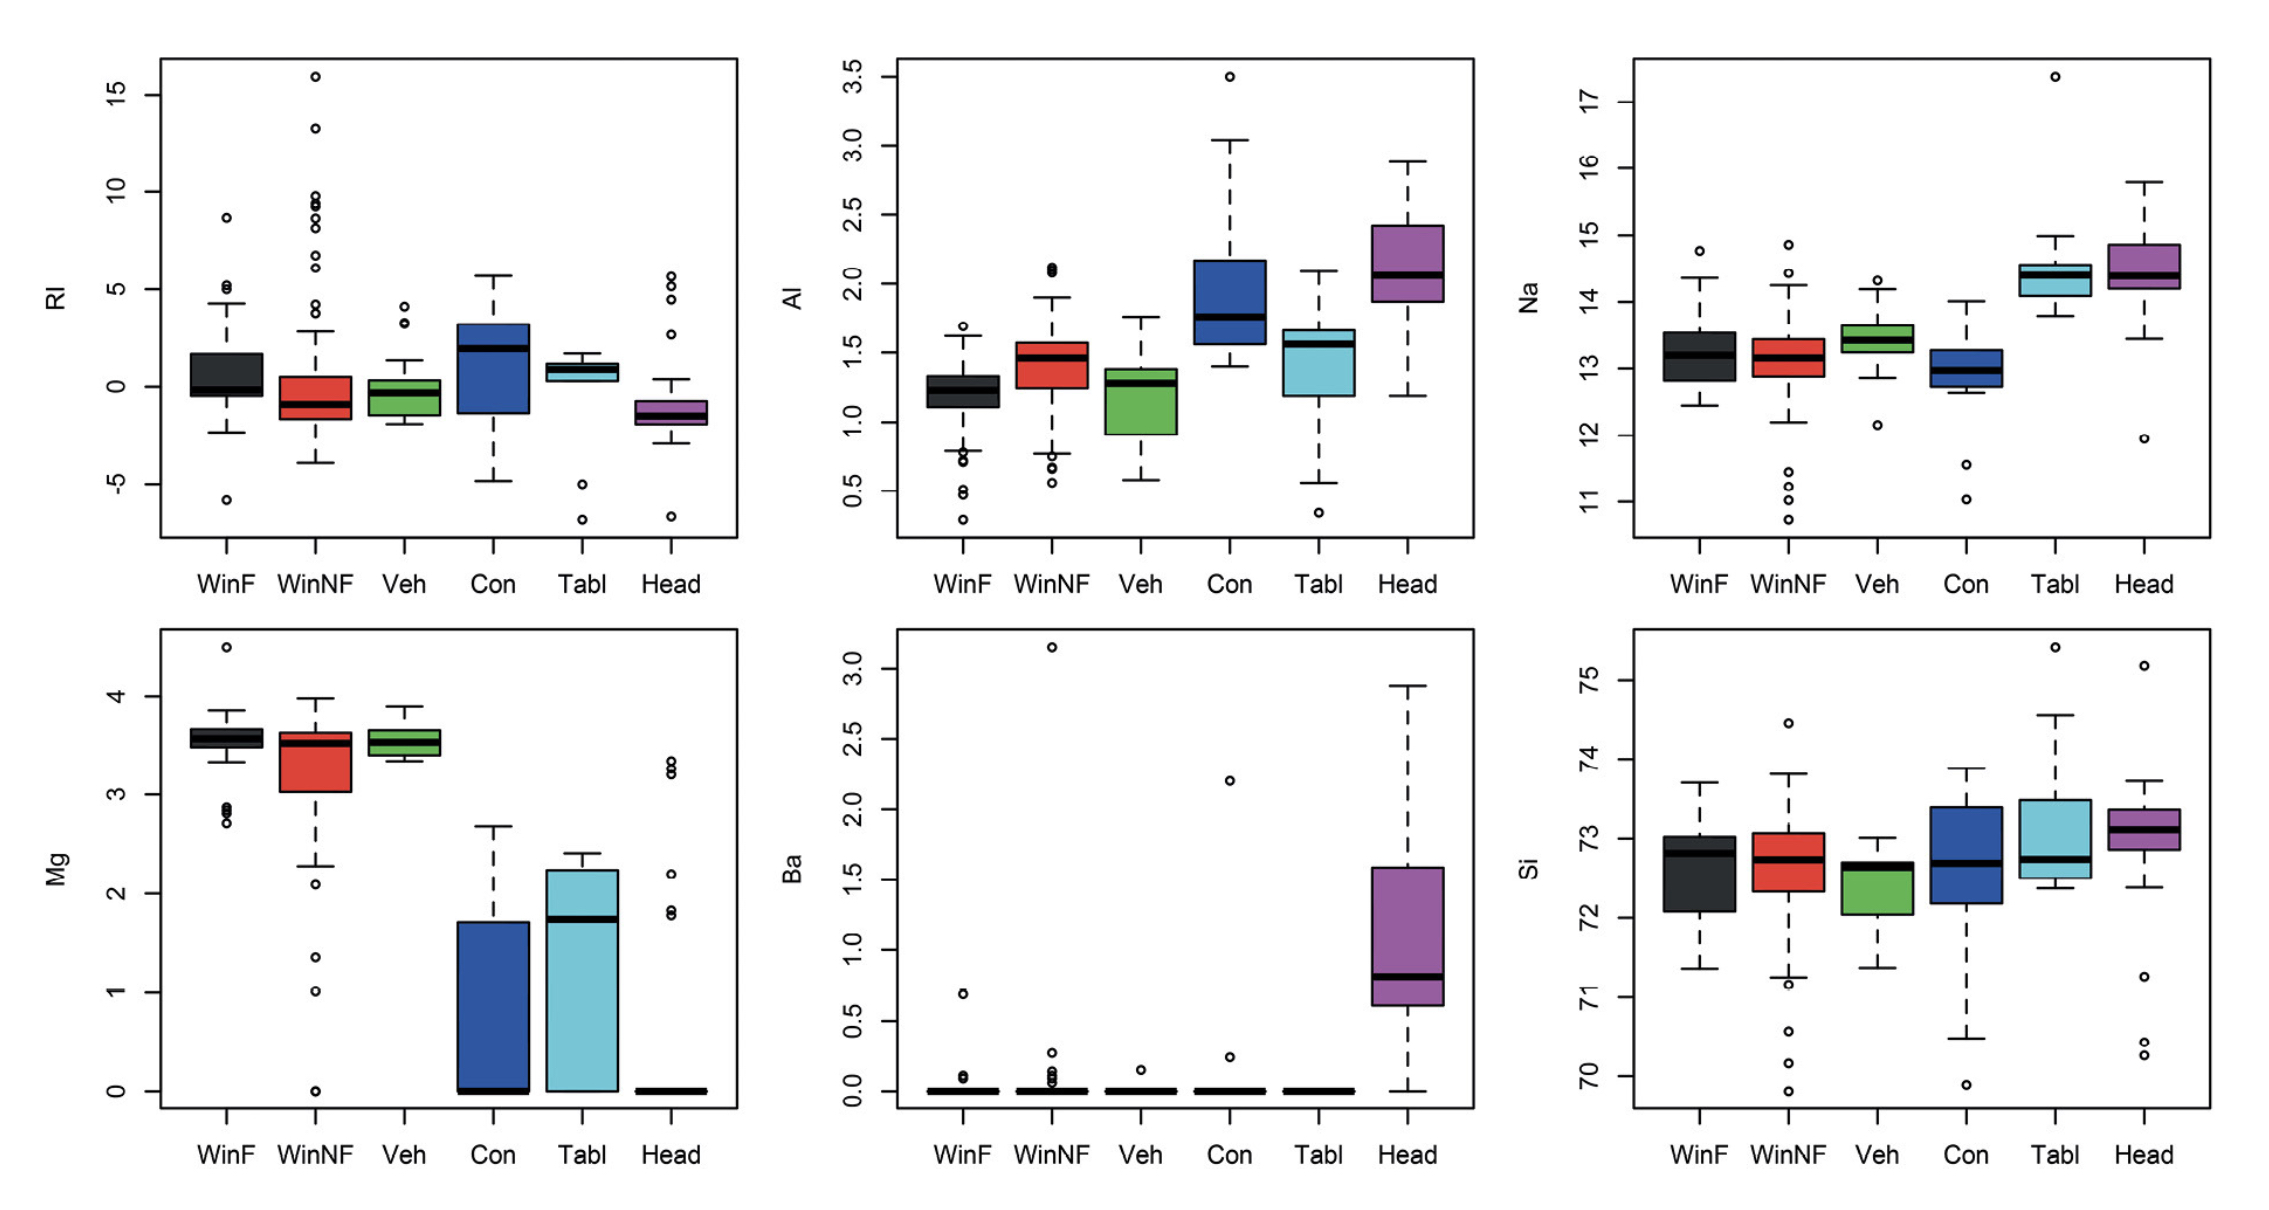
\includegraphics[scale=0.15]{figures/glass}
              
 \end{figure}


\end{frame}
%----------------------------------------------------------------------%
\begin{frame}[fragile]
\frametitle{K-Nearest Neighbors}

\begin{itemize}
  \item Units matter

\begin{itemize}
 \item Since distance is measured on the raw $x$ values, units matter.
 \item As we did for regularization, we will standarized observations.
 \item \texttt{R scale} function does this, i.e., convert columns to mean-zero sd-one
\end{itemize}
\end{itemize}
\bigskip
\begin{scriptsize}
\begin{Shaded}
\begin{Highlighting}[]
\NormalTok{x \textless{}{-}}\StringTok{ }\KeywordTok{scale}\NormalTok{(fgl[,}\DecValTok{1}\OperatorTok{:}\DecValTok{9}\NormalTok{]) }\CommentTok{\# column 10 is the class label}
\KeywordTok{apply}\NormalTok{(x,}\DecValTok{2}\NormalTok{,sd) }\CommentTok{\# see ?apply}
\end{Highlighting}
\end{Shaded}
\end{scriptsize}
\begin{tiny}
\begin{verbatim}
## RI Na Mg Al Si  K Ca Ba Fe 
##  1  1  1  1  1  1  1  1  1
\end{verbatim}
\end{tiny}
\end{frame}
%----------------------------------------------------------------------%
\begin{frame}[fragile]
\frametitle{K-Nearest Neighbors}

\begin{itemize}
  \item Before running \texttt{Knn}
  \begin{itemize}
    \item Make sure you have numeric matrices of training data $x$ values, with labels $y$
    \item Also need to provide new $test$ values where you would like to predict
    \item Note that there's no model do fit, \texttt{Knn}, just counts neighbors for each observation in \texttt{test}
  \end{itemize}
  
\end{itemize}
\begin{scriptsize}
\begin{Shaded}
\begin{Highlighting}[]
\KeywordTok{set.seed}\NormalTok{(}\DecValTok{1010101}\NormalTok{)}
\NormalTok{test \textless{}{-}}\StringTok{ }\KeywordTok{sample}\NormalTok{(}\DecValTok{1}\OperatorTok{:}\DecValTok{214}\NormalTok{,}\DecValTok{10}\NormalTok{)}
\NormalTok{nearest1 \textless{}{-}}\StringTok{ }\KeywordTok{knn}\NormalTok{(}\DataTypeTok{train=}\NormalTok{x[}\OperatorTok{{-}}\NormalTok{test,], }\DataTypeTok{test=}\NormalTok{x[test,], }\DataTypeTok{cl=}\NormalTok{fgl}\OperatorTok{$}\NormalTok{type[}\OperatorTok{{-}}\NormalTok{test], }\DataTypeTok{k=}\DecValTok{1}\NormalTok{)}
\NormalTok{nearest5 \textless{}{-}}\StringTok{ }\KeywordTok{knn}\NormalTok{(}\DataTypeTok{train=}\NormalTok{x[}\OperatorTok{{-}}\NormalTok{test,], }\DataTypeTok{test=}\NormalTok{x[test,], }\DataTypeTok{cl=}\NormalTok{fgl}\OperatorTok{$}\NormalTok{type[}\OperatorTok{{-}}\NormalTok{test], }\DataTypeTok{k=}\DecValTok{5}\NormalTok{)}
\KeywordTok{data.frame}\NormalTok{(fgl}\OperatorTok{$}\NormalTok{type[test],nearest1,nearest5)}
\end{Highlighting}
\end{Shaded}
\end{scriptsize}
\begin{tiny}

\begin{verbatim}
##    fgl.type.test. nearest1 nearest5
## 1            WinF     WinF    WinNF
## 2            Head     Head     Head
## 3           WinNF    WinNF    WinNF
## 4            WinF     WinF     WinF
## 5           WinNF    WinNF    WinNF
## 6           WinNF    WinNF    WinNF
## 7            Head      Con      Con
## 8            Head    WinNF    WinNF
## 9           WinNF    WinNF    WinNF
## 10          WinNF     WinF     WinF
\end{verbatim}
\end{tiny}
\end{frame}

%----------------------------------------------------------------------%
\subsection{Logit}
%----------------------------------------------------------------------%
\begin{frame}[fragile]
\frametitle{Logit Demo}

\begin{scriptsize}
\begin{Shaded}
\begin{Highlighting}[]
\KeywordTok{set.seed}\NormalTok{(}\DecValTok{101010}\NormalTok{) }\CommentTok{\#sets a seed }
\NormalTok{credit\textless{}{-}}\KeywordTok{readRDS}\NormalTok{(}\StringTok{"credit\_class.rds"}\NormalTok{)}
\CommentTok{\#70\% train}
\NormalTok{indic\textless{}{-}}\KeywordTok{sample}\NormalTok{(}\DecValTok{1}\OperatorTok{:}\KeywordTok{nrow}\NormalTok{(credit),}\KeywordTok{floor}\NormalTok{(.}\DecValTok{7}\OperatorTok{*}\KeywordTok{nrow}\NormalTok{(credit)))}
\CommentTok{\#Partition the sample}
\NormalTok{train\textless{}{-}credit[indic,]}
\NormalTok{test\textless{}{-}credit[}\OperatorTok{{-}}\NormalTok{indic,]}
\KeywordTok{head}\NormalTok{(credit)}
\end{Highlighting}
\end{Shaded}
\end{scriptsize}
\begin{tiny}
\begin{verbatim}
##   Default duration amount installment age  history      purpose foreign  rent
## 1       0        6   1169           4  67 terrible goods/repair foreign FALSE
## 2       1       48   5951           2  22     poor goods/repair foreign FALSE
## 3       0       12   2096           2  49 terrible          edu foreign FALSE
## 4       0       42   7882           2  45     poor goods/repair foreign FALSE
## 5       1       24   4870           3  53     poor       newcar foreign FALSE
## 6       0       36   9055           2  35     poor          edu foreign FALSE
\end{verbatim}
\end{tiny}
\begin{scriptsize}


\begin{Shaded}
\begin{Highlighting}[]
\KeywordTok{dim}\NormalTok{(credit)}
\end{Highlighting}
\end{Shaded}
\end{scriptsize}
\begin{tiny}
\begin{verbatim}
## [1] 1000    9
\end{verbatim}
\end{tiny}


\end{frame}
%----------------------------------------------------------------------%
\begin{frame}[fragile]
\frametitle{Logit Demo}

\begin{scriptsize}
\begin{Shaded}
\begin{Highlighting}[]
\NormalTok{mylogit \textless{}{-}}\StringTok{ }\KeywordTok{glm}\NormalTok{(Default}\OperatorTok{\textasciitilde{}}\NormalTok{duration }\OperatorTok{+}\StringTok{ }\NormalTok{amount }\OperatorTok{+}\StringTok{ }\NormalTok{installment }\OperatorTok{+}\StringTok{ }\NormalTok{age }
              \OperatorTok{+}\StringTok{ }\KeywordTok{factor}\NormalTok{(history) }\OperatorTok{+}\StringTok{ }\KeywordTok{factor}\NormalTok{(purpose) }\OperatorTok{+}\StringTok{ }\KeywordTok{factor}\NormalTok{(foreign) }\OperatorTok{+}\StringTok{ }\KeywordTok{factor}\NormalTok{(rent), }
              \DataTypeTok{data =}\NormalTok{ train, }\DataTypeTok{family =} \StringTok{"binomial"}\NormalTok{)}
\KeywordTok{summary}\NormalTok{(mylogit)}
\end{Highlighting}
\end{Shaded}
\end{scriptsize}
\begin{tiny}
\begin{verbatim}
## 
## ...
## 
## Coefficients:
##                               Estimate Std. Error z value Pr(>|z|)    
## (Intercept)                 -3.285e-01  5.597e-01  -0.587 0.557264    
## duration                     1.625e-02  9.538e-03   1.704 0.088369 .  
## amount                       1.518e-04  4.325e-05   3.511 0.000447 ***
## installment                  3.335e-01  9.216e-02   3.619 0.000296 ***
## age                         -1.762e-02  8.851e-03  -1.990 0.046554 *  
## factor(history)poor         -1.212e+00  3.126e-01  -3.876 0.000106 ***
## factor(history)terrible     -1.989e+00  3.552e-01  -5.598 2.17e-08 ***
## factor(purpose)usedcar      -1.813e+00  4.067e-01  -4.459 8.23e-06 ***
## factor(purpose)goods/repair -7.163e-01  2.254e-01  -3.177 0.001486 ** 
## factor(purpose)edu           1.207e-01  3.858e-01   0.313 0.754450    
## factor(purpose)biz          -9.862e-01  3.440e-01  -2.867 0.004147 ** 
## factor(foreign)german       -2.057e+00  8.213e-01  -2.505 0.012254 *  
## factor(rent)TRUE             7.554e-01  2.355e-01   3.208 0.001337 ** 
## ---
## Signif. codes:  0 '***' 0.001 '**' 0.01 '*' 0.05 '.' 0.1 ' ' 1
## 
## ...
\end{verbatim}
\end{tiny}
\end{frame}
%----------------------------------------------------------------------%
\begin{frame}[fragile]
\frametitle{Logit Demo}

\begin{scriptsize}
\begin{Shaded}
\begin{Highlighting}[]
\NormalTok{test}\OperatorTok{$}\NormalTok{phat\textless{}{-}}\StringTok{ }\KeywordTok{predict}\NormalTok{(mylogit, test, }\DataTypeTok{type=}\StringTok{"response"}\NormalTok{)}
\NormalTok{test}\OperatorTok{$}\NormalTok{Default\_hat\textless{}{-}}\KeywordTok{ifelse}\NormalTok{(test}\OperatorTok{$}\NormalTok{phat}\OperatorTok{\textgreater{}}\NormalTok{.}\DecValTok{5}\NormalTok{,}\DecValTok{1}\NormalTok{,}\DecValTok{0}\NormalTok{)}
\KeywordTok{with}\NormalTok{(test,}\KeywordTok{prop.table}\NormalTok{(}\KeywordTok{table}\NormalTok{(Default,Default\_hat)))}
\end{Highlighting}
\end{Shaded}

\end{scriptsize}

\begin{columns}[T] % align columns
\begin{column}{.42\textwidth}
  

\begin{scriptsize}
\begin{verbatim}
##        Default_hat
## Default          0          1
##       0 0.63666667 0.06666667
##       1 0.22666667 0.07000000
\end{verbatim}
\end{scriptsize}

\end{column}  
\hfill
\begin{column}{.48\textwidth}

 \begin{figure}[H] \centering
            \captionsetup{justification=centering}
              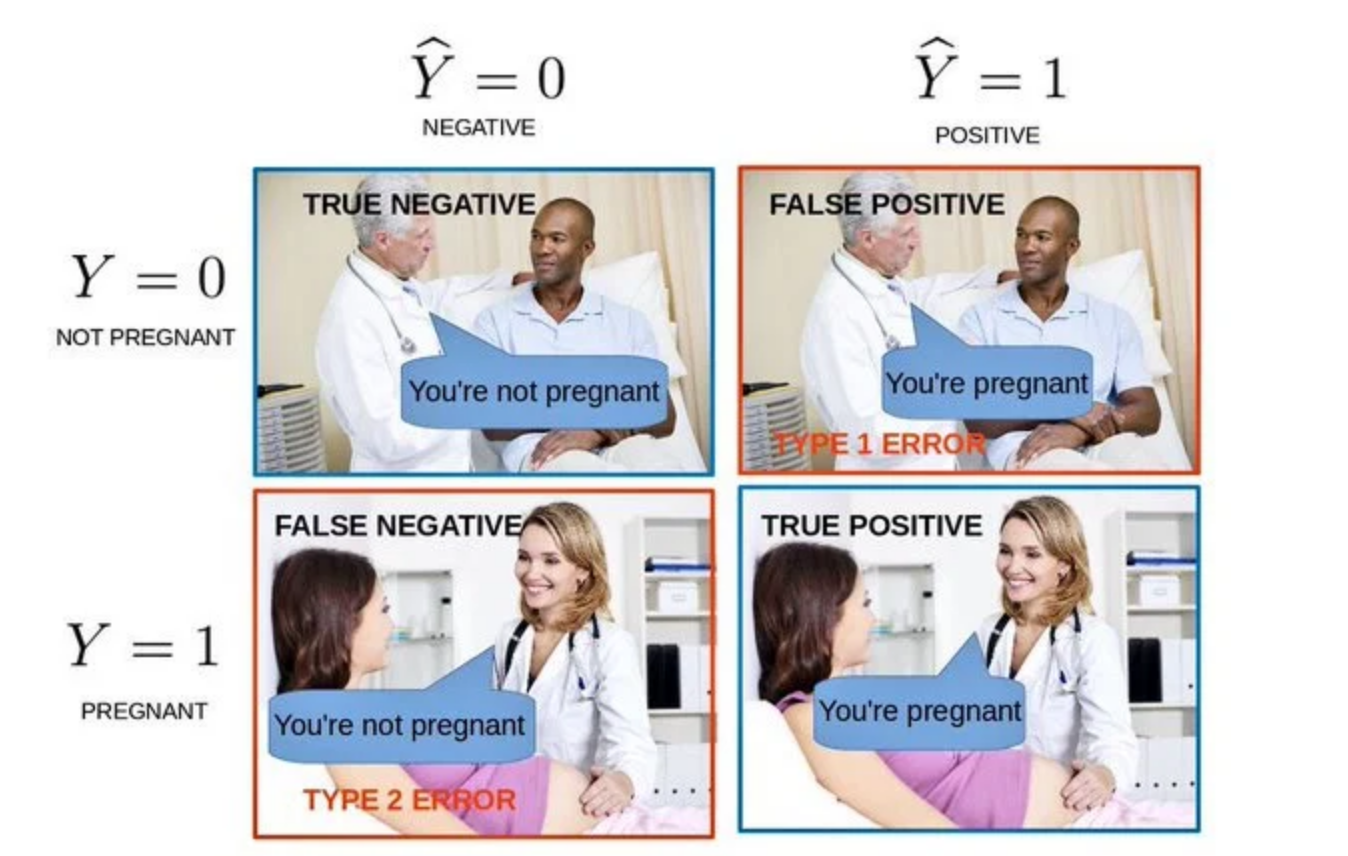
\includegraphics[scale=0.3]{figures/confusion_matrix}                           
 \end{figure}

\end{column}
\end{columns}

\end{frame}
%----------------------------------------------------------------------%
\subsection{LDA}
%----------------------------------------------------------------------%
\begin{frame}[fragile]
\frametitle{LDA: Demo}
\begin{scriptsize}
\begin{align}
    p(y=1) = \frac{\sum_{i=1}^n 1[y_i=1]}{N}
  \end{align}


\begin{Shaded}
\begin{Highlighting}[]
\NormalTok{p1\textless{}{-}}\KeywordTok{sum}\NormalTok{(train}\OperatorTok{$}\NormalTok{Default)}\OperatorTok{/}\KeywordTok{dim}\NormalTok{(train)[}\DecValTok{1}\NormalTok{]}
\NormalTok{p1}
\end{Highlighting}
\end{Shaded}
\begin{verbatim}
## [1] 0.3014286
\end{verbatim}
\end{scriptsize}
\begin{scriptsize}
\begin{align}
\hat{\mu}_k=\frac{1}{n_k}\sum_{i:y_i=k}x_i
\end{align}


\begin{Shaded}
\begin{Highlighting}[]
\NormalTok{mu1\textless{}{-}}\KeywordTok{mean}\NormalTok{(train}\OperatorTok{$}\NormalTok{duration[train}\OperatorTok{$}\NormalTok{Default}\OperatorTok{==}\DecValTok{1}\NormalTok{])}
\NormalTok{mu1}
\end{Highlighting}
\end{Shaded}

\begin{verbatim}
## [1] 24.78673
\end{verbatim}

\begin{Shaded}
\begin{Highlighting}[]
\NormalTok{mu0\textless{}{-}}\KeywordTok{mean}\NormalTok{(train}\OperatorTok{$}\NormalTok{duration[train}\OperatorTok{$}\NormalTok{Default}\OperatorTok{==}\DecValTok{0}\NormalTok{])}
\NormalTok{mu0}
\end{Highlighting}
\end{Shaded}

\begin{verbatim}
## [1] 19.79346
\end{verbatim}
\end{scriptsize}

\end{frame}
%----------------------------------------------------------------------%
\begin{frame}[fragile]
\frametitle{LDA: Demo}


\begin{align}
\hat{\sigma}^2 = \frac{1}{N-K} \sum_{k=1}^K \sum_{i:y_i=k} (x_i -\hat{\mu}_k)^2
\end{align}

\begin{scriptsize}
\begin{Shaded}
\begin{Highlighting}[]
\NormalTok{g1\textless{}{-}}\KeywordTok{sum}\NormalTok{((train}\OperatorTok{$}\NormalTok{duration[train}\OperatorTok{$}\NormalTok{Default}\OperatorTok{==}\DecValTok{1}\NormalTok{]}\OperatorTok{{-}}\NormalTok{mu1)}\OperatorTok{\^{}}\DecValTok{2}\NormalTok{)}
\NormalTok{g0\textless{}{-}}\KeywordTok{sum}\NormalTok{((train}\OperatorTok{$}\NormalTok{duration[train}\OperatorTok{$}\NormalTok{Default}\OperatorTok{==}\DecValTok{0}\NormalTok{]}\OperatorTok{{-}}\NormalTok{mu0)}\OperatorTok{\^{}}\DecValTok{2}\NormalTok{)}


\NormalTok{sigma\textless{}{-}}\KeywordTok{sqrt}\NormalTok{((g1}\OperatorTok{+}\NormalTok{g0)}\OperatorTok{/}\NormalTok{(}\KeywordTok{dim}\NormalTok{(train)[}\DecValTok{1}\NormalTok{]}\OperatorTok{{-}}\DecValTok{2}\NormalTok{))}
\end{Highlighting}
\end{Shaded}
\end{scriptsize}

\begin{align}
\hat{f}_k \sim N(\hat{\mu}_k,\hat{\sigma})
\end{align}

\begin{scriptsize}
\begin{Shaded}
\begin{Highlighting}[]
\NormalTok{f1\textless{}{-}}\KeywordTok{dnorm}\NormalTok{(test}\OperatorTok{$}\NormalTok{duration,}\DataTypeTok{mean=}\NormalTok{mu1,}\DataTypeTok{sd=}\NormalTok{sigma)}
\NormalTok{f0\textless{}{-}}\KeywordTok{dnorm}\NormalTok{(test}\OperatorTok{$}\NormalTok{duration,}\DataTypeTok{mean=}\NormalTok{mu0,}\DataTypeTok{sd=}\NormalTok{sigma)}
\end{Highlighting}
\end{Shaded}
\end{scriptsize}

\end{frame}
%----------------------------------------------------------------------%
\begin{frame}[fragile]
\frametitle{LDA: Demo}
\begin{scriptsize}


\begin{Shaded}
\begin{Highlighting}[]
\KeywordTok{library}\NormalTok{(}\StringTok{"MASS"}\NormalTok{)     }\CommentTok{\# LDA}
\NormalTok{lda\_simple \textless{}{-}}\StringTok{ }\KeywordTok{lda}\NormalTok{(Default}\OperatorTok{\textasciitilde{}}\NormalTok{duration, }\DataTypeTok{data =}\NormalTok{ train)}
\NormalTok{lda\_simple\_pred\textless{}{-}}\KeywordTok{predict}\NormalTok{(lda\_simple,test)}
\KeywordTok{names}\NormalTok{(lda\_simple\_pred)}
\end{Highlighting}
\end{Shaded}
\end{scriptsize}
\begin{tiny}
\begin{verbatim}
## [1] "class"     "posterior" "x"
\end{verbatim}
\end{tiny}


\begin{scriptsize}
\begin{Shaded}
\begin{Highlighting}[]
\NormalTok{posteriors\textless{}{-}}\KeywordTok{data.frame}\NormalTok{(lda\_simple\_pred}\OperatorTok{$}\NormalTok{posterior)}
\NormalTok{posteriors}\OperatorTok{$}\NormalTok{hand\textless{}{-}f1}\OperatorTok{*}\NormalTok{p1}\OperatorTok{/}\NormalTok{(f1}\OperatorTok{*}\NormalTok{p1}\OperatorTok{+}\NormalTok{f0}\OperatorTok{*}\NormalTok{(}\DecValTok{1}\OperatorTok{{-}}\NormalTok{p1))}
\KeywordTok{head}\NormalTok{(posteriors)}
\end{Highlighting}
\end{Shaded}



\begin{verbatim}
##           X0        X1      hand
## 1  0.8013656 0.1986344 0.1986344
## 3  0.7668614 0.2331386 0.2331386
## 14 0.6861792 0.3138208 0.3138208
## 16 0.6861792 0.3138208 0.3138208
## 28 0.7668614 0.2331386 0.2331386
## 33 0.7283950 0.2716050 0.2716050
\end{verbatim}
\end{scriptsize}
\end{frame}

%----------------------------------------------------------------------%
\subsection{ROC}
%----------------------------------------------------------------------%
\begin{frame}[fragile]
\frametitle{Roc Demo}
\begin{scriptsize}

\begin{Shaded}
\begin{Highlighting}[]
\KeywordTok{library}\NormalTok{(}\StringTok{"ROCR"}\NormalTok{) }\CommentTok{\#Roc}

\NormalTok{mylogit \textless{}{-}}\StringTok{ }\KeywordTok{glm}\NormalTok{(Default}\OperatorTok{\textasciitilde{}}\NormalTok{duration }\OperatorTok{+}\StringTok{ }\NormalTok{amount }\OperatorTok{+}\StringTok{ }\NormalTok{installment }\OperatorTok{+}\StringTok{ }\NormalTok{age }
                \OperatorTok{+}\StringTok{ }\KeywordTok{factor}\NormalTok{(history) }\OperatorTok{+}\StringTok{ }\KeywordTok{factor}\NormalTok{(purpose) }\OperatorTok{+}\StringTok{ }\KeywordTok{factor}\NormalTok{(foreign) }\OperatorTok{+}\StringTok{ }\KeywordTok{factor}\NormalTok{(rent), }
                \DataTypeTok{data =}\NormalTok{ train, }\DataTypeTok{family =} \StringTok{"binomial"}\NormalTok{)}
\NormalTok{test}\OperatorTok{$}\NormalTok{phat\textless{}{-}}\StringTok{ }\KeywordTok{predict}\NormalTok{(mylogit, test, }\DataTypeTok{type=}\StringTok{"response"}\NormalTok{)}
\NormalTok{pred \textless{}{-}}\StringTok{ }\KeywordTok{prediction}\NormalTok{(test}\OperatorTok{$}\NormalTok{phat, test}\OperatorTok{$}\NormalTok{Default)}
\NormalTok{roc\_ROCR \textless{}{-}}\StringTok{ }\KeywordTok{performance}\NormalTok{(pred,}\StringTok{"tpr"}\NormalTok{,}\StringTok{"fpr"}\NormalTok{)}
\KeywordTok{plot}\NormalTok{(roc\_ROCR, }\DataTypeTok{main =} \StringTok{"ROC curve"}\NormalTok{, }\DataTypeTok{colorize =}\NormalTok{ T)}
\KeywordTok{abline}\NormalTok{(}\DataTypeTok{a =} \DecValTok{0}\NormalTok{, }\DataTypeTok{b =} \DecValTok{1}\NormalTok{)}
\end{Highlighting}
\end{Shaded}
\end{scriptsize}


 \begin{figure}[H] \centering
            \captionsetup{justification=centering}
              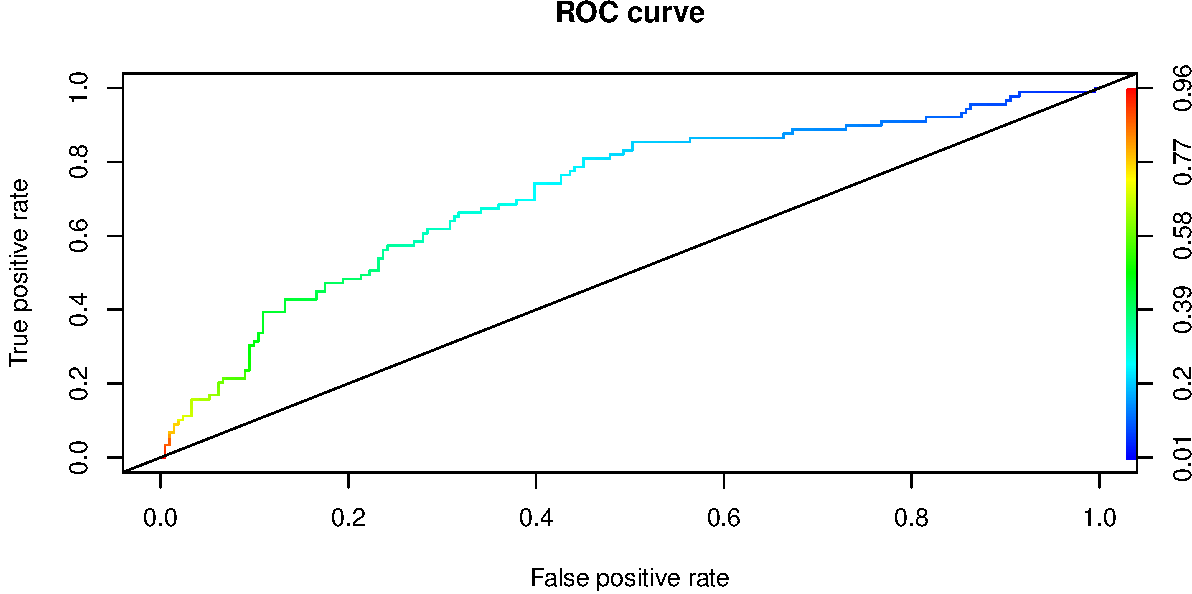
\includegraphics[scale=0.4]{figures/unnamed-chunk-7-1.pdf}
 \end{figure}

\end{frame}
%----------------------------------------------------------------------%
\begin{frame}[fragile]
\frametitle{Roc Demo}


 \begin{figure}[H] \centering
            \captionsetup{justification=centering}
              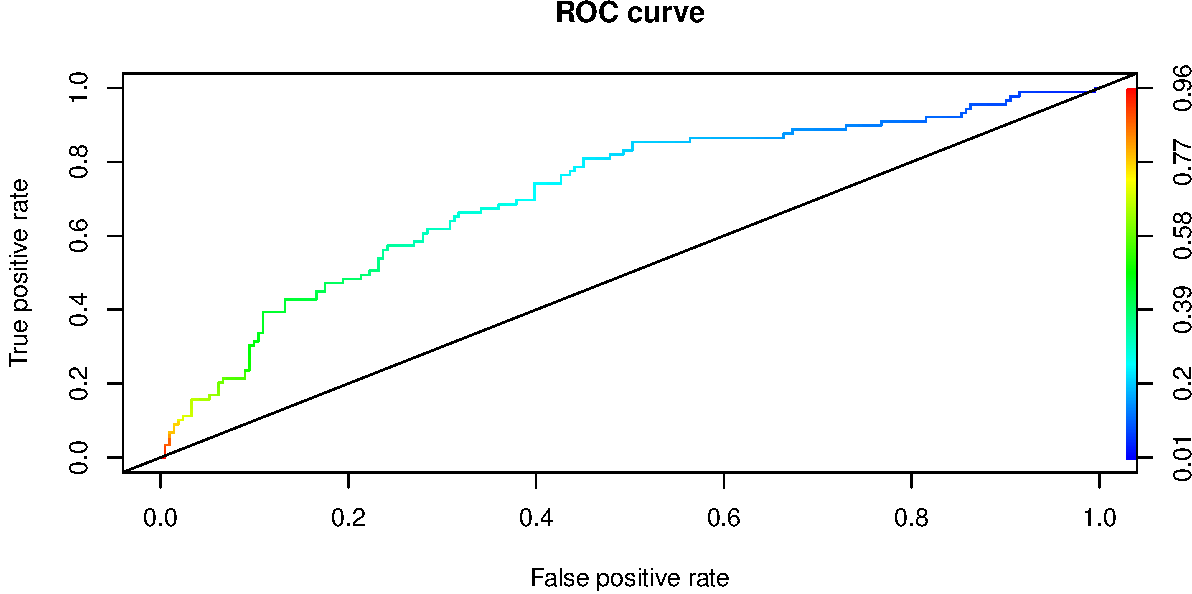
\includegraphics[scale=0.4]{figures/unnamed-chunk-7-1.pdf}
 \end{figure}

\begin{scriptsize}
\begin{Shaded}
\begin{Highlighting}[]
\NormalTok{auc\_ROCR \textless{}{-}}\StringTok{ }\KeywordTok{performance}\NormalTok{(pred, }\DataTypeTok{measure =} \StringTok{"auc"}\NormalTok{)}
\NormalTok{auc\_ROCR}\OperatorTok{@}\NormalTok{y.values[[}\DecValTok{1}\NormalTok{]]}
\end{Highlighting}
\end{Shaded}

\begin{verbatim}
## [1] 0.714415
\end{verbatim}
\end{scriptsize}

\end{frame}
%----------------------------------------------------------------------%
\begin{frame}[fragile]
\frametitle{Roc Demo}

\begin{scriptsize}
\begin{Shaded}
\begin{Highlighting}[]
\NormalTok{mylda \textless{}{-}}\StringTok{ }\KeywordTok{lda}\NormalTok{(Default}\OperatorTok{\textasciitilde{}}\NormalTok{duration }\OperatorTok{+}\StringTok{ }\NormalTok{amount }\OperatorTok{+}\StringTok{ }\NormalTok{installment }\OperatorTok{+}\StringTok{ }\NormalTok{age , }\DataTypeTok{data =}\NormalTok{ train)}
\NormalTok{mylda}
\end{Highlighting}
\end{Shaded}
\end{scriptsize}

\begin{tiny}

\begin{verbatim}
## Call:
## lda(Default ~ duration + amount + installment + age, data = train)
## 
## Prior probabilities of groups:
##         0         1 
## 0.6985714 0.3014286 
## 
## Group means:
##   duration   amount installment      age
## 0 19.79346 3062.888    2.885481 36.40900
## 1 24.78673 4057.791    3.109005 33.85782
## 
## Coefficients of linear discriminants:
##                       LD1
## duration     0.0296041361
## amount       0.0002055164
## installment  0.4821242957
## age         -0.0386710882
\end{verbatim}
\end{tiny}

\end{frame}
%----------------------------------------------------------------------%
\begin{frame}[fragile]
\frametitle{Roc Demo}
\begin{scriptsize}


\begin{Shaded}
\begin{Highlighting}[]
\NormalTok{phat\_mylda\textless{}{-}}\StringTok{ }\KeywordTok{predict}\NormalTok{(mylda, test, }\DataTypeTok{type=}\StringTok{"response"}\NormalTok{)}
\NormalTok{pred\_mylda \textless{}{-}}\StringTok{ }\KeywordTok{prediction}\NormalTok{(phat\_mylda}\OperatorTok{$}\NormalTok{posterior[,}\DecValTok{2}\NormalTok{], test}\OperatorTok{$}\NormalTok{Default)}

\NormalTok{roc\_mylda \textless{}{-}}\StringTok{ }\KeywordTok{performance}\NormalTok{(pred\_mylda,}\StringTok{"tpr"}\NormalTok{,}\StringTok{"fpr"}\NormalTok{)}
\KeywordTok{plot}\NormalTok{(roc\_mylda, }\DataTypeTok{main =} \StringTok{"ROC curve"}\NormalTok{, }\DataTypeTok{colorize =}\NormalTok{ T)}
\KeywordTok{abline}\NormalTok{(}\DataTypeTok{a =} \DecValTok{0}\NormalTok{, }\DataTypeTok{b =} \DecValTok{1}\NormalTok{)}
\end{Highlighting}
\end{Shaded}


\begin{figure}[H] \centering
            \captionsetup{justification=centering}
              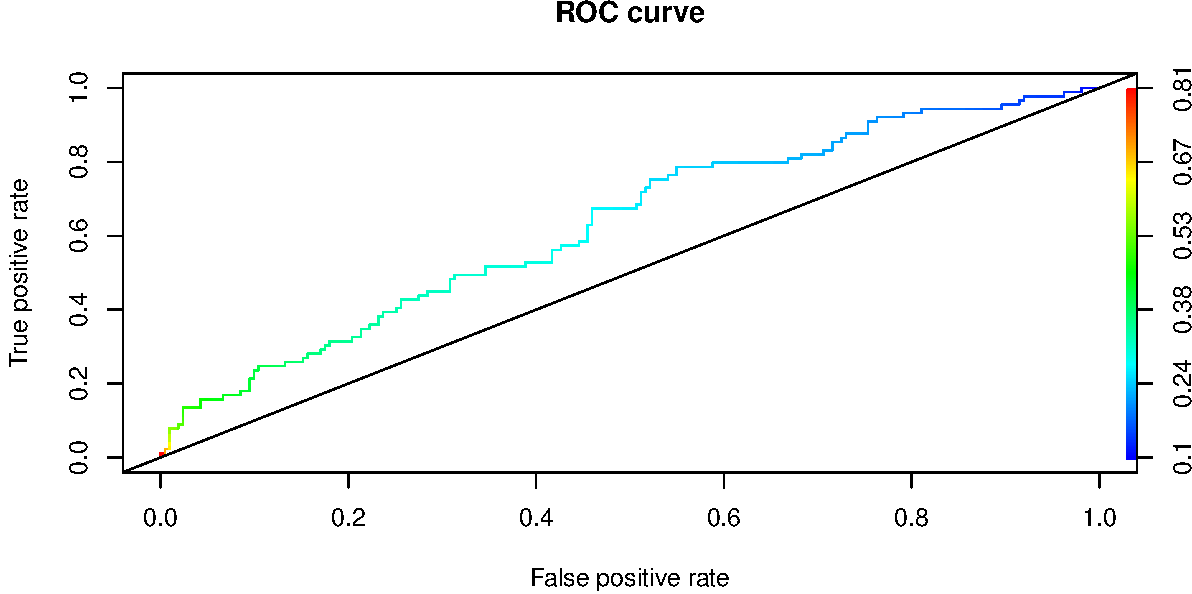
\includegraphics[scale=0.4]{figures/unnamed-chunk-10-1.pdf}
 \end{figure}
\end{scriptsize}
\end{frame}
%----------------------------------------------------------------------%
\begin{frame}[fragile]
\frametitle{Roc Demo}

\begin{scriptsize}
\begin{Shaded}
\begin{Highlighting}[]
\KeywordTok{plot}\NormalTok{(roc\_ROCR, }\DataTypeTok{main =} \StringTok{"ROC curve"}\NormalTok{, }\DataTypeTok{colorize =} \OtherTok{FALSE}\NormalTok{, }\DataTypeTok{col=}\StringTok{"red"}\NormalTok{)}
\KeywordTok{plot}\NormalTok{(roc\_mylda,}\DataTypeTok{add=}\OtherTok{TRUE}\NormalTok{, }\DataTypeTok{colorize =} \OtherTok{FALSE}\NormalTok{, }\DataTypeTok{col=}\StringTok{"blue"}\NormalTok{)}
\KeywordTok{abline}\NormalTok{(}\DataTypeTok{a =} \DecValTok{0}\NormalTok{, }\DataTypeTok{b =} \DecValTok{1}\NormalTok{)}
\end{Highlighting}
\end{Shaded}
\end{scriptsize}

\begin{figure}[H] \centering
            \captionsetup{justification=centering}
              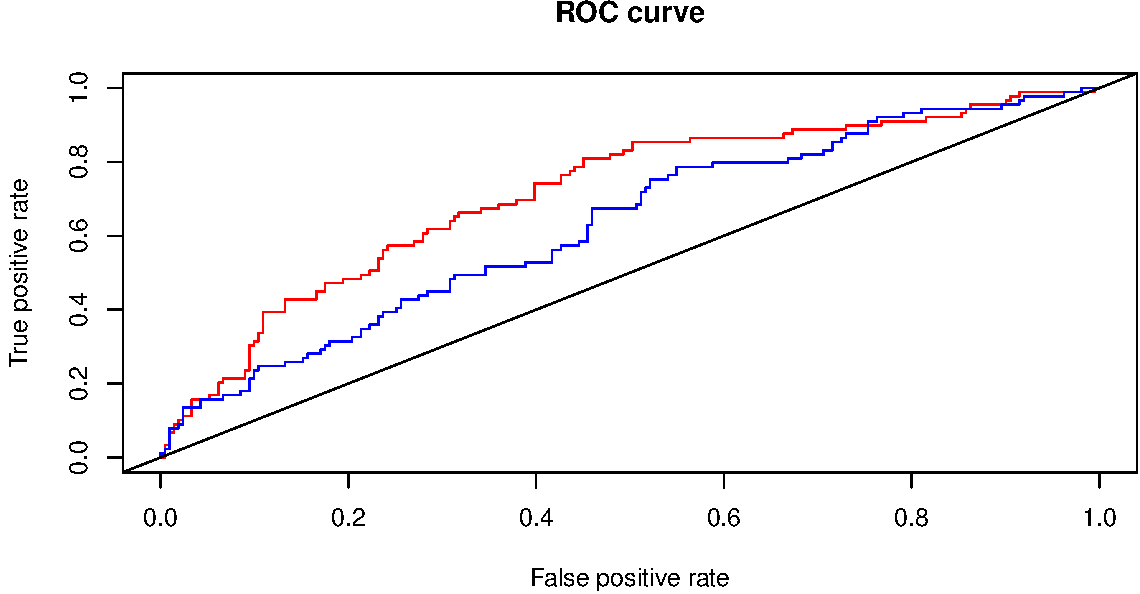
\includegraphics[scale=0.4]{figures/unnamed-chunk-11-1.pdf}
 \end{figure}

\end{frame}
%----------------------------------------------------------------------%
\begin{frame}[fragile]
\frametitle{Roc Demo}
\begin{itemize}
  \item Area under the curve (AUC)

\end{itemize}
\begin{scriptsize}
\begin{Shaded}
\begin{Highlighting}[]
\NormalTok{auc\_ROCR \textless{}{-}}\StringTok{ }\KeywordTok{performance}\NormalTok{(pred, }\DataTypeTok{measure =} \StringTok{"auc"}\NormalTok{)}
\NormalTok{auc\_ROCR\_lda\_simple \textless{}{-}}\StringTok{ }\KeywordTok{performance}\NormalTok{(pred\_mylda, }\DataTypeTok{measure =} \StringTok{"auc"}\NormalTok{)}
\NormalTok{auc\_ROCR}\OperatorTok{@}\NormalTok{y.values[[}\DecValTok{1}\NormalTok{]]}
\end{Highlighting}
\end{Shaded}

\begin{verbatim}
## [1] 0.714415
\end{verbatim}


\begin{Shaded}
\begin{Highlighting}[]
\NormalTok{auc\_ROCR\_lda\_simple}\OperatorTok{@}\NormalTok{y.values[[}\DecValTok{1}\NormalTok{]]}
\end{Highlighting}
\end{Shaded}


\begin{verbatim}
## [1] 0.6291602
\end{verbatim}
\end{scriptsize}

\end{frame}




%----------------------------------------------------------------------%
%----------------------------------------------------------------------%
\end{document}
%----------------------------------------------------------------------%
%----------------------------------------------------------------------%

